\documentclass[final,hyperref={pdfpagelabels=false}]{beamer}
%%% THEME FOR THE POSTER %%%
\usetheme{LTS5}

%%% PACKAGES DECLARATION
%%%%%%%%%%%%%%%%%%%%%%%%%%%%%%%%%%%%%%%%%%%%%%%%%%%
% Signal Processing Laboratory (LTS5) - EPFL      %
% LaTeX beamposter template                       %
% Authors:                                        %
%   D. Perdios – dimitris.perdios@epfl.ch         %
%   A. Besson – adrien.besson@epfl.ch             %
% v0.1 - 08.05.17                                 %
% Typeset configuration: pdfLaTeX + Biber         %
%%%%%%%%%%%%%%%%%%%%%%%%%%%%%%%%%%%%%%%%%%%%%%%%%%%

% Poster related package
\usepackage[orientation=portrait,size=a0,scale=1.4]{beamerposter} % Use the beamerposter package for laying out the poster with a portrait orientation and an a0 paper size
\usepackage{textpos}

% Typesetting
\usepackage[T1]{fontenc}
\usepackage[utf8]{inputenc}
\usepackage[english]{babel}
\usepackage{lmodern} % latin modern font
\usepackage{exscale} % scaling extension of the math fonts
%\usepackage[scaled]{helvet} % sans serif typo
\usepackage{csquotes} % pro­vides ad­vanced fa­cil­i­ties for in­line and dis­play quo­ta­tions (better to load when using biblatex)
\usepackage{textcomp} % pro­vide many text sym­bols (such as baht, bul­let, copy­right, mu­si­cal­note, onequar­ter, sec­tion, and yen), in the TS1 en­cod­ing
%\usepackage{setspace}
%	\onehalfspacing % 1.5 linespaceing (already in CLS)
%\usepackage{fancyhdr} % pro­vides ex­ten­sive fa­cil­i­ties, both for con­struct­ing head­ers and foot­ers, and for con­trol­ling their use
\usepackage{siunitx} % SI units system typset
%\usepackage{enumitem}
%	\setlist[enumerate]{label*=\arabic*.,topsep=5pt,partopsep=0pt,parsep=0pt,itemsep=2pt}
%	\setlist[itemize]{topsep=5pt,partopsep=0pt,parsep=0pt,itemsep=2pt}
\usepackage{fontawesome} % high quality web icons

% Math
\usepackage{amsmath}
\usepackage{amsfonts}
\usepackage{amssymb}
\usepackage{amsthm}
\usepackage{bm}
\usepackage{mathdots} % mathfonts for vdots
%\usefonttheme[onlymath]{serif} % uncomment for serif math equations

% Figures
\usepackage{graphicx}
	\graphicspath{{figures/}}
\usepackage{xcolor}
\usepackage[font=small, labelfont=bf, format=plain, labelsep=space, figurename=Figure, tablename=Table]{caption}
\usepackage[labelfont=sf, labelformat=parens, labelsep=space]{subcaption}

% Tables
%\usepackage{multirow}
\usepackage{longtable} % use \linebreak instead of \\ in headers to avoid a bug with longtables (or longtabu) across two pages
\usepackage{booktabs} % the pack­age en­hances the qual­ity of ta­bles (toprule, bottomrule, etc.)
\usepackage{tabu}
%	\renewcommand{\arraystretch}{1.3}

% Codes
\usepackage{listings}
%	Some style definitions
\lstdefinestyle{lstLaTeX}{
	aboveskip=0pt,
	belowskip=0pt,
    language=[LaTeX]TeX,
    breaklines=true,
    basicstyle=\ttfamily\scriptsize,
%    keywordstyle=\color{blue},
%    identifierstyle=\color{magenta},
}
\lstdefinestyle{lstinlineLaTeX}{
	style=lstLaTeX, 		% uses the LaTeX listings style
    basicstyle=\ttfamily,	% only redefines the basicstyle
}
\lstdefinestyle{lstC}{
	aboveskip=0pt,
	belowskip=0pt,
	breaklines=true,
%	xleftmargin=\parindent,
	language=C,
	showstringspaces=false,
	basicstyle=\scriptsize\ttfamily,
	keywordstyle=\bfseries\color{green!40!black},
	commentstyle=\itshape\color{purple!40!black},
	identifierstyle=\color{blue},
	stringstyle=\color{orange},
}

% Algorithms
\usepackage{algorithm}
\usepackage{algpseudocode} % The algorithmicx package provides many possibilities to customize the layout of algorithms.
	\algrenewcommand\textproc{\small\MakeUppercase} %BEAMER ONLY: Latin Modern Sans fonts don't have small caps
%TODO: Check if can be put in .sty
	
% Others
\usepackage{beamerbasetheorems}
\usepackage{calc}
\usepackage{lipsum}
\usepackage{silence}
% Filter warnings issued by package biblatex starting with "Patching footnotes failed"
	\WarningFilter{biblatex}{Patching footnotes failed}

% Videos
%\usepackage[draft]{media9}
%\usepackage{media9}

% Emoji (thanks slide)
%\usepackage[nointegrals]{wasysym} % new characters (smiley)

% Biblatex
\usepackage[
	backend=biber,
	bibstyle=ieee,
	citestyle=ieee
]{biblatex} % style=ieee loads both, bibstyle and citestyle

% References and urls
% hyperref already loaded by beamer internally
\usepackage{url}
\usepackage{bookmark} % Im­ple­ments a new book­mark (out­line) or­ga­ni­za­tion for pack­age hy­per­ref
%%%%%%%%%%%%%%%%%%%%%%%%%%%%%%%%%%%%%%%%%%%%%%%%%%%
% Signal Processing Laboratory (LTS5) - EPFL      %
% LaTeX beamer template                           %
% Authors:                                        %
%   D. Perdios – dimitris.perdios@epfl.ch         %
%   A. Besson – adrien.besson@epfl.ch             %
% v0.1 - 18.11.16                                 %
% Typeset configuration: pdfLaTeX + Biber         %
%%%%%%%%%%%%%%%%%%%%%%%%%%%%%%%%%%%%%%%%%%%%%%%%%%%


% Specific package declarations

%%% COMMANDS %%%
%%%%%%%%%%%%%%%%%%%%%%%%%%%%%%%%%%%%%%%%%%%%%%%%%%%
% Signal Processing Laboratory (LTS5) - EPFL      %
% LaTeX beamposter template                       %
% Authors:                                        %
%   D. Perdios – dimitris.perdios@epfl.ch         %
%   A. Besson – adrien.besson@epfl.ch             %
% v0.1 - 08.05.17                                 %
% Typeset configuration: pdfLaTeX + Biber         %
%%%%%%%%%%%%%%%%%%%%%%%%%%%%%%%%%%%%%%%%%%%%%%%%%%%


% New command used to create a blank column

\newcommand{\AddBlankColumn}[1]{
	\begin{column}{#1}\end{column}
}

%%% SIZES OF THE MARGINS AND COLUMNS

%%% CUSTOM MAKETITLE COMMAND %%%
\newlength{\LogoWidthLeft}
\settowidth{\LogoWidthLeft}{
\includegraphics[height=\LogoHeight]{logos/lts5_logo.pdf}}
\newlength{\LogoWidthRight}
\settowidth{\LogoWidthRight}{
\includegraphics[height=\LogoHeight]{logos/epfl_logo.pdf}}
\setlength{\titlewidth}{\LeftColumnWidth + \RightColumnWidth + \BlankColumnWidthCenter- \LogoWidthLeft - \LogoWidthRight - \BlankColumnWidthLeft-\BlankColumnWidthRight}
\newsavebox{\titlebox}
\newlength{\myposterheight}
\renewcommand{\maketitle}{%
	\savebox{\titlebox}{%
		\hspace{\BlankColumnWidthLeft}
		\begin{minipage}{\LogoWidthLeft}%
			
\includegraphics[height=\LogoHeight]{logos/basp_logo.png}
			\vspace{\LogoSkip}
			\centering
			
\includegraphics[height=\LogoHeight]{logos/lts5_logo.pdf}
		\end{minipage} 
		\begin{minipage}{\titlewidth}%
			\centering
			\LARGE\inserttitle \leavevmode\\%
			\normalsize\insertauthor \leavevmode\\%
			\small\insertinstitute %
		\end{minipage} 
		\begin{minipage}{\LogoWidthRight}%
			
\includegraphics[height=\LogoHeight]{logos/epfl_logo.pdf}
			\vspace{\LogoSkip}
			\centering
			
\includegraphics[height=\LogoHeight]{logos/lts5_logo.pdf}
		\end{minipage}
		\hspace{\BlankColumnWidthRight}
	}%
	\settoheight{\titleheight}{\usebox{\titlebox}}
	\setlength{\myposterheight}{0.97\textheight - \titleheight - \TitleColumnSpace}
	\usebox{\titlebox}
}



%%% TITLE CONTENT %%%
%%%%%%%%%%%%%%%%%%%%%%%%%%%%%%%%%%%%%%%%%%%%%%%%%%%
% Signal Processing Laboratory (LTS5) - EPFL      %
% LaTeX beamposter template                       %
% Authors:                                        %
%   D. Perdios – dimitris.perdios@epfl.ch         %
%   A. Besson – adrien.besson@epfl.ch             %
% v0.1 - 08.05.17                                 %
% Typeset configuration: pdfLaTeX + Biber         %
%%%%%%%%%%%%%%%%%%%%%%%%%%%%%%%%%%%%%%%%%%%%%%%%%%%


%%%%%%%%%%%%%% TITLE PAGE
\title[EPFLIBM]{On an analytical, spatially-varying, point-spread-function for ultrasound imaging}

% CASE1: SINGLE AUTHOR
\author[short-author]{ % [short-author] is optional (used with \insertshortauthor)
	\href{mailto:lucien.roquette@epfl.ch}{Lucien Roquette\inst{1}},
	\href{mailto:mathieu.simeoni@epfl.ch}{Mathieu Simeoni\inst{1}}
	\href{mailto:mathieu.simeoni@epfl.ch}{Paul Hurley\inst{1}}
	\href{mailto:adrien.besson@epfl.ch}{Adrien Besson\inst{2}}	
}

\institute{
	\inst{1}IBM Zurich Research Laboratory, Rüschlikon \\
	\href{http://lts5www.epfl.ch}{\inst{2}Signal Processing Laboratory (LTS5)}, \href{http://www.epfl.ch/index.en.html}{\'Ecole Polytechnique F\'ed\'erale de Lausanne}
}

%%% BIBLIOGRAPHY %%%
\addbibresource{example.bib}

\begin{document}

	\begin{frame}[t] 
	
	% Create the title
	\maketitle
		
	\vspace{\TitleColumnSpace}
	
	\begin{columns}[t] 
		
		\AddBlankColumn{\BlankColumnWidthLeft} % Empty spacer column
		
		\begin{column}{\LeftColumnWidth} % The first column
			\vbox to \myposterheight{%
%----------------------------------------------------------------------------------------
%	OBJECTIVES
%----------------------------------------------------------------------------------------

\begin{block}{Introduction and objectives}
	
	\begin{itemize}
		\item The point spread function (PSF), \ie the response of a system to a point source, is a measure of the quality of an ultrasound~(US) imager
		\item PSF usuallycrudely estimated by assuming spatial-invariance, or estimated via simulation, coupled with reconstruction algorithms 
		\item Lack of an analytical formulation inhibits many applications ranging from optimization of apodization schemes, to array-design to and deconvolution algorithms
		\item We propose an analytical formulation of the PSF and use it for deconvolution of US images
	\end{itemize}
	
\end{block}
\vfill

%----------------------------------------------------------------------------------------
%	INTRODUCTION
%----------------------------------------------------------------------------------------

\begin{block}{Notations and data-model}
	
	\begin{columns} % Subdivide the first main column
		\begin{column}{.54\textwidth} % The first subdivided column within the first main column
			\begin{itemize}
				\item Notations:
				\begin{itemize}
					\item 1D probe composed of $N_{el}$ transducer elements located at $\bm{r}_i$
					\item $m_i\left(t\right)$ signal received at $i^{th}$ element
					\item Medium $\Omega \subset \mathbb{R}^2$ characterized by its tissue reflectivity function~(TRF) $\gamma \left(\vect{r}\right)$
					\item $b \left(\vect{r}, \vect{r}_i\right)$ spatially varying attenuation term  
					\item $h\left(t\right)$ is the elementary waveform
				\end{itemize}
			\end{itemize}
		\end{column}
		
		\begin{column}{.43\textwidth} % The second subdivided column within the first main column
			\centering
			\begin{figure}
				{\footnotesize
					\begin{tikzpicture}[%
scale=\columnwidth/15cm,
>={Stealth[inset=0pt]},
thick,
transducer/.style = {scale=\columnwidth/15cm, shape=rectangle, draw=black, fill=transducer-color, thick, minimum height=\transducerHeight cm, minimum width=\transducerWidth cm, inner sep=0pt},
measurement/.style = {decorate, decoration=snake, color=measurement-color, thick}
]
% Help grid
%	\draw[help lines] (0,0) grid[step=0.5cm] (20, -15);

% Transducers
\coordinate (pos_td1) at (\transducerInitXPos, {0.5*\transducerHeight});
\coordinate (xoff_td) at (\transducerXOffset, 0);

\foreach \pt in {1,...,\transducerNumb}
\node[transducer] (td\pt) at ($ (pos_td1) + \pt*(xoff_td) - (xoff_td) $) {};

% Scatterer
\pgfmathsetmacro{\scatPointX}{9.6} % use axes_orig
\pgfmathsetmacro{\scatPointZ}{6.2}

% http://tex.stackexchange.com/questions/3594/tikz-node-labels-more-below-than-below#3596
%	\node[fill, shape=circle, minimum size=0.1cm, inner sep=0cm, outer sep=0cm, color=scatterer-color, label=below:\textcolor{scatterer-color}{$\left(\vect{r}, \gamma\left(\vect{r}\right)\right)$}] (scatterer_point) at (\scatPointX, -\scatPointZ) {}; % NOT exactly 0.1cm radius..., not exactly the correct "below" distance
\node[fill, shape=circle, minimum size=0.1cm, inner sep=0cm, outer sep=0cm, color=scatterer-color] (scatterer_point) at (\scatPointX, -\scatPointZ) {};
\fill[color=scatterer-color] (scatterer_point) circle[radius=0.1] node[below]{$\left(\vect{r}, \gamma\left(\vect{r}\right)\right)$};

% Measurements
%	\pgfmathsetmacro{\pt}{7}
%	\pgfmathsetmacro{\tdPosX}{\transducerInitXPos+(\pt-1)*\transducerXOffset}
%	\pgfmathsetmacro{\rForward}{\scatPointZ} % z
%	\pgfmathsetmacro{\rBackward}{sqrt((\scatPointX - \tdPosX)^2 + \scatPointZ^2)}
%	\pgfmathsetmacro{\rTot}{\rForward+\rBackward}
%	\pgfmathsetmacro{\tPulseCenter}{\rTot/1 - 11.5}
%	
%	\pgfmathsetmacro{\tStart}{\measurementLength - \tPulseCenter - 1/2}
%	\pgfmathsetmacro{\tEnd}{\tStart + 1}
%	\draw[domain=0:\tStart, thick, smooth, variable=\t, red] plot ({\tdPosX+0*\t}, {\t+\transducerHeight});
%	\draw[domain=0:1, thick, smooth, variable=\t, red]  plot ({\tdPosX + 0.5*(1-cos((2*pi*\t) r))*0.4*\transducerWidth*sin(3*2*pi*(\t) r)},{\transducerHeight+\tStart+\t});
%	\draw[domain=\tEnd:\measurementLength, thick, smooth, variable=\t, red] plot ({\tdPosX+0*\t}, {\t+\transducerHeight});
%	%	\node[above] at (\tdPosX, \measurementLength + \transducerHeight) {\rotatebox{90}{\textcolor{blue}{\tPulseCenter}}};

\begin{scope}[on background layer]
\foreach \pt in {1,...,\transducerNumb}
{
	\pgfmathsetmacro{\tdPosX}{\transducerInitXPos+(\pt-1)*\transducerXOffset}
	\pgfmathsetmacro{\rForward}{\scatPointZ} % z
	\pgfmathsetmacro{\rBackward}{sqrt((\scatPointX - \tdPosX)^2 + \scatPointZ^2)}
	\pgfmathsetmacro{\rTot}{\rForward+\rBackward}
	\pgfmathsetmacro{\tPulseCenter}{\rTot/1 - 11.5}
	
	\pgfmathsetmacro{\tStart}{\measurementLength - \tPulseCenter - 1/2}
	\pgfmathsetmacro{\tEnd}{\tStart + 1}
	\draw[domain=0:\tStart, thick, smooth, variable=\t, measurement-color] plot ({\tdPosX+0*\t}, {\t+\transducerHeight});
	\draw[domain=0:1, thick, smooth, variable=\t, measurement-color]  plot ({\tdPosX + 0.5*(1-cos((2*pi*\t) r))*0.4*\transducerWidth*sin(3*2*pi*(\t) r)},{\transducerHeight+\tStart+\t});
	\draw[domain=\tEnd:\measurementLength, thick, smooth, variable=\t, measurement-color] plot ({\tdPosX+0*\t}, {\t+\transducerHeight});
	%		\node[above] at (\tdPosX, \measurementLength + \transducerHeight) {\rotatebox{90}{\textcolor{blue}{\tPulseCenter}}};
	
	% Measurement label
	%		\draw[] (\tdPosX, \transducerHeight) -- node[midway, sloped, below]{$m_i\left(t\right)$} (\tdPosX, {\tStart+\transducerHeight});
	\ifdefstrequal{\pt}{\transducerLabeled}{%
		\fill[color=measurement-color] (\tdPosX, {\tStart+\transducerHeight}) circle[radius=0] node[below left]{\rotatebox{90}{$m_i\left(t\right)$}};
		% COULD USE \path without option for an invisible path
	}{}
	
}
\end{scope}

% Labels for transducer and measurement
\pgfmathsetmacro{\tdPosX}{\transducerInitXPos+(\transducerLabeled-1)*\transducerXOffset}
\node[above] at (td\transducerLabeled) {$\vect{r}_i$};
%	\node[above] at (\tdPosX, \measurementLength + \transducerHeight) {\rotatebox{90}{\textcolor{measurement-color}{$m_i\left(t\right)$}}};


% Axes
\pgfmathsetmacro{\vertAxisX}{\transducerInitXPos - \axesOffset}
\pgfmathsetmacro{\transducerLength}{(\transducerNumb-1)*\transducerXOffset}
\coordinate (axes_orig) at (\vertAxisX, 0);
\coordinate (x_axis_end) at ({\transducerInitXPos + \transducerLength + \axesOffset}, 0);
\coordinate (z_axis_end) at (\vertAxisX, {-\scatPointZ - \axesOffset});
\coordinate (t_axis_start) at (\vertAxisX, \transducerHeight + \measurementLength);
\coordinate (t_axis_end) at (\vertAxisX, \transducerHeight + \axesOffset);

\draw[<->] (x_axis_end) node[right] {$x$} -- (axes_orig) -- (z_axis_end) node[below] {$z$};
\draw[->] (t_axis_start) -- (t_axis_end) node[below] {$t$};

% Plane wave: Wavefront and transmit time of flight
\pgfmathsetmacro{\thetaPW}{15} % degree
\pgfmathsetmacro{\thetaLabXOffset}{2.2}
\pgfmathsetmacro{\PWaveFrontStartX}{\transducerInitXPos}
\pgfmathsetmacro{\PWaveFrontStartZ}{\transducerHeight}
\pgfmathsetmacro{\PWaveFrontEndX}{\transducerInitXPos+\transducerLength}
\pgfmathsetmacro{\PWaveFrontEndZ}{\transducerHeight+sin(\thetaPW)*\transducerLength}
\coordinate (pw_wavefront_start) at (\PWaveFrontStartX, \PWaveFrontStartZ);
\coordinate (pw_wavefront_end) at (\PWaveFrontEndX, \PWaveFrontEndZ);
\coordinate (pw_wavefront_scat_proj) at ($(pw_wavefront_start)!(scatterer_point)!(pw_wavefront_end)$);

%	Transmit wavefront
\begin{scope}[on background layer]
\draw[dashed, wavefront-color, thick, name path=pw_wavefront_path] (pw_wavefront_start) -- (pw_wavefront_end);
%TODO: use clip on an extended path line
\end{scope}
%	%		Angle
%	\begin{scope}[on background layer]
%		\draw[wavefront-color, thin] ({\PWaveFrontStartX+\thetaLabXOffset},{\PWaveFrontStartZ}) arc[start angle=0, end angle=\thetaPW, radius=\thetaLabXOffset] node[midway, right]{$\theta$};
%	\end{scope}

% 		Wavefront label
\path[name path=data_right_limit_path] ({\transducerInitXPos+\transducerLength}, 0) -- ({\transducerInitXPos+\transducerLength}, {\transducerHeight+\measurementLength});
%\fill[name intersections={of=pw_wavefront_path and data_right_limit_path, by = pw_wavefront_label_point}] (pw_wavefront_label_point) circle[radius=0] node[right, align=center, wavefront-color]{``wavefront''}; % specificying the key align= allows to add newlines

%	Transmit time of flight
\draw[->, wavefront-color] (pw_wavefront_scat_proj) -- node[midway, sloped, below] {$t_{Tx}\left(\vect{r}\right)$} (scatterer_point);

%	% Diverging wave: Wavefront and transmit time of flight
%	\pgfmathsetmacro{\DWVirtualPointX}{\transducerInitXPos + 3}
%	\pgfmathsetmacro{\DWVirtualPointZ}{1.2*\measurementLength + \transducerHeight}
%	\pgfmathsetmacro{\DWBetaAngleRadius}{0.35cm}
%	
%	%	Virtual point
%	\node[fill, shape=circle, minimum size=0.1cm, inner sep=0cm, outer sep=0cm, color=wavefront-color] (dw_virtual_point) at (\DWVirtualPointX, \DWVirtualPointZ) {};
%	\fill[color=wavefront-color] (dw_virtual_point) circle[radius=0] node[above]{$\vect{r}_n$};
%	
%	%	Wavefront
%	\begin{scope}[on background layer]
%%		\clip (\transducerInitXPos, \transducerHeight) rectangle ({\transducerInitXPos+\transducerLength}, {\transducerHeight, \measurementLength});
%		\begin{scope} % just for the clip
%			\clip (\transducerInitXPos, \transducerHeight) rectangle ({\transducerInitXPos+\transducerLength}, {\transducerHeight+\measurementLength});
%%		\path[draw, thick, wavefront-color, name path=dw_wavefront_path] (dw_virtual_point) circle [radius={\DWVirtualPointZ-\transducerHeight}];
%			\draw[dashed, thick, wavefront-color, name path=dw_wavefront_path] (dw_virtual_point) circle [radius={\DWVirtualPointZ-\transducerHeight}];
%		\end{scope}
%	\end{scope}
%	
%	% 		Wavefront label
%	\path[name path=data_right_limit_path] ({\transducerInitXPos+\transducerLength}, 0) -- ({\transducerInitXPos+\transducerLength}, {\transducerHeight+\measurementLength});
%	\fill[name intersections={of=dw_wavefront_path and data_right_limit_path, by = dw_wavefront_label_point}] (dw_wavefront_label_point) circle[radius=0] node[right, align=center, wavefront-color]{``wavefront''}; % specificying the key align= allows to add newlines
%	
%	%	Intersection on the circular wavefront
%	\path[name path=dw_virtual_point_to_scatterer] (dw_virtual_point) -- (scatterer_point);
%	
%	% 	Transmit time of flight
%	\fill[name intersections={of=dw_wavefront_path and dw_virtual_point_to_scatterer, by = dw_point_on_wavefront}] (dw_point_on_wavefront) circle[radius=0];
%%	\draw[-, wavefront-color] [name intersections={of=dw_wavefront_path and dw_virtual_point_to_scatterer, by = dw_point_on_wavefront}] (dw_virtual_point) -- (dw_point_on_wavefront);
%	\draw[dotted, wavefront-color] (dw_virtual_point) -- (dw_point_on_wavefront);
%	\draw[->, wavefront-color](dw_point_on_wavefront) -- node[midway, sloped, below] {$t_{Tx}\left(\vect{r}\right)$} (scatterer_point);
%	\begin{scope}[on background layer]
%		\path[name path=transducer_height_path] (\vertAxisX, \transducerHeight) -- ({\transducerInitXPos+\transducerLength+\axesOffset}, \transducerHeight);
%		%	Angle
%		\fill[red, name intersections={of=transducer_height_path and dw_virtual_point_to_scatterer, by = dw_beta_base_point}] (dw_beta_base_point) circle[radius=0cm];
%		\pic[pic text=$\beta$, draw, wavefront-color, thin, angle radius=\DWBetaAngleRadius, angle eccentricity=1.4] {angle= dw_virtual_point--dw_beta_base_point--td1};
%	\end{scope}
%
%	
% Receive time for flight
\draw[->, wavefront-color] (scatterer_point) -- node[midway, sloped, below] {$\frac{\|\vect{r}-\vect{r}_i\|_2}{c}$} (td\transducerLabeled.south);
%	
%	% 1-D conic (ellipse)
%	\coordinate (dw_ellipse_focus1) at (dw_virtual_point);
%	\coordinate (dw_ellipse_focus2) at (td\transducerLabeled);
%	\begin{scope} % just for the clip
%		\clip (\transducerInitXPos, 0) rectangle ({\transducerInitXPos+\transducerLength}, -\domainZMax);
%		\ellipsebyfoci{draw, conic-color, name path=dw_conic_path}{dw_ellipse_focus1}{dw_ellipse_focus2}{16.5}
%	\end{scope}
%	%	Conic label
%	\newcommand*{\conicTextLabel}{``ellipse''}
%	\newcommand*{\conicMathLabel}{$\left[
%		x\left(\alpha\right), z\left(\alpha\right)\right]^T$}
%	\pgfmathsetmacro{\vertGridX}{\transducerInitXPos+9*\transducerXOffset}
%	\path[name path=domain_vert_path] (\vertGridX, 0) -- (\vertGridX, -\domainZMax);
%	\fill[name intersections={of=dw_conic_path and domain_vert_path, by = dw_conic_label_point}] (dw_conic_label_point) circle[radius=0] node[right, align=center, conic-color]{\conicTextLabel}; % specificying the key align= allows to add newlines
%	
%	% Insonified domain (i.e. Grid)
%	% http://tex.stackexchange.com/questions/45808/tikz-grid-lines
%	\begin{scope}[on background layer]
%		\draw[step=1, very thin, color=domain-color] (\domainXMin, -\domainZMin) grid (\domainXMax, -\domainZMax);
%	\end{scope}
%	
%	% 	Discretization
%	\pgfmathsetmacro{\discretizedPointLabeledNumb}{3}
%%	\newcommand*{\discretizedPointMathLabel}{$\left[
%%		x\left(\alpha^p\right), z\left(\alpha^p\right)\right]^T$}
%	\newcommand*{\discretizedPointMathLabel}{$\vect{r}\left(\alpha^p\right)$}
%	%		TODO: set a gridNumb
%	\foreach \gridVert in {1,...,\transducerNumb}
%	{
%		\pgfmathsetmacro{\vertGridX}{\domainXMin+(\gridVert-1)*\domainDxOffset}
%		\path[name path=domain_vert_path] (\vertGridX, -\domainZMin) -- (\vertGridX, -\domainZMax);
%		\fill[name intersections={of=dw_conic_path and domain_vert_path, by = discretized_conic_point}] (discretized_conic_point) circle[radius=0.1];
%		
%		\ifdefstrequal{\gridVert}{\discretizedPointLabeledNumb}{%
%			\fill (discretized_conic_point) circle[radius=0] node[above right]{\discretizedPointMathLabel};
%			% COULD USE \path without option for an invisible path
%		}{}
%	}
%	
%	%	Grid spacing
%	\newcommand*{\spacingLabelOffset}{7pt}
%	\pgfmathsetmacro{\domainDxIndexX}{8} % 1 - 10
%	\pgfmathsetmacro{\domainDxIndexZ}{8} % 1 - 8
%	\pgfmathsetmacro{\domainDzIndexX}{10} % 1 - 10
%	\pgfmathsetmacro{\domainDzIndexZ}{6} % 1 - 8
%	\pgfmathsetmacro{\domainDxOneX}{\domainXMin+(\domainDxIndexX-1)*\domainDxOffset}
%	\pgfmathsetmacro{\domainDxTwoX}{\domainXMin+(\domainDxIndexX)*\domainDxOffset}
%	\pgfmathsetmacro{\domainDxOneZ}{-\domainZMin-(\domainDxIndexZ-1)*\domainDzOffset}
%	\pgfmathsetmacro{\domainDxTwoZ}{-\domainZMin-(\domainDxIndexZ-1)*\domainDzOffset}
%	\pgfmathsetmacro{\domainDzOneX}{\domainXMin+(\domainDzIndexX-1)*\domainDzOffset}
%	\pgfmathsetmacro{\domainDzTwoX}{\domainXMin+(\domainDzIndexX-1)*\domainDzOffset}
%	\pgfmathsetmacro{\domainDzOneZ}{-\domainZMin-(\domainDzIndexZ-1)*\domainDzOffset}
%	\pgfmathsetmacro{\domainDzTwoZ}{-\domainZMin-(\domainDzIndexZ)*\domainDzOffset}
%%	\fill[red] (\domainDxOneX, \domainDxOneZ) circle[radius=0.1];
%%	\fill[blue] (\domainDxTwoX, \domainDxTwoZ) circle[radius=0.1];
%%	\fill[red] (\domainDzOneX, \domainDzOneZ) circle[radius=0.1];
%%	\fill[blue] (\domainDzTwoX, \domainDzTwoZ) circle[radius=0.1];
%	\coordinate (domain_dx_one) at (\domainDxOneX, \domainDxOneZ);
%	\coordinate (domain_dx_two) at (\domainDxTwoX, \domainDxTwoZ);
%	\coordinate (domain_dz_one) at (\domainDzOneX, \domainDzOneZ);
%	\coordinate (domain_dz_two) at (\domainDzTwoX, \domainDzTwoZ);
%	\draw[|-|, thin] ($ (domain_dx_one) - (0, \spacingLabelOffset) $) -- node[below] {$\Delta x$} ($ (domain_dx_two) - (0, \spacingLabelOffset) $);
%	\draw[|-|, thin] ($ (domain_dz_two) + (\spacingLabelOffset, 0) $) -- node[midway, sloped, below] {$\Delta z$} ($ (domain_dz_one) + (\spacingLabelOffset, 0) $);
%	
%	%	Inter-element spacing
%	\pgfmathsetmacro{\transducerDxiOne}{2}
%	\pgfmathsetmacro{\transducerDxiTwo}{3}
%	\draw[|-|, thin] ($ (td\transducerDxiOne.south) - (0, \spacingLabelOffset) $) -- node[below] {$\Delta \vect{r}_i$} ($ (td\transducerDxiTwo.south) - (0, \spacingLabelOffset) $);
%	
%	
\end{tikzpicture}}
				%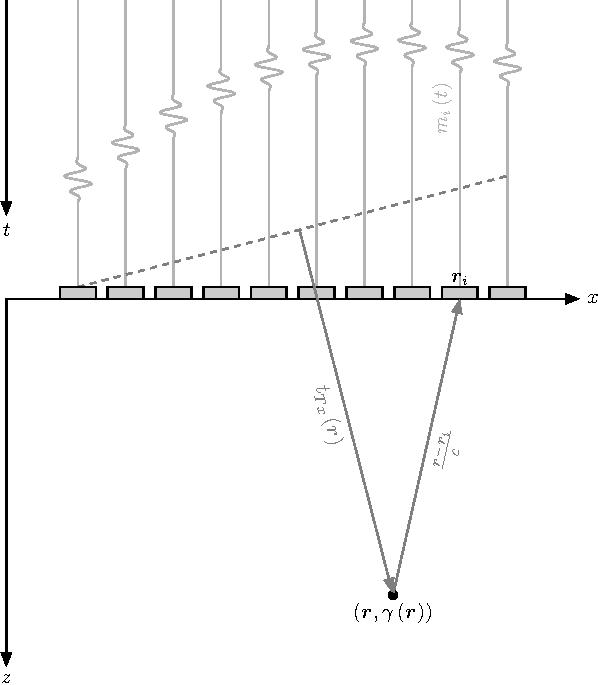
\includegraphics[width=0.9\linewidth]{tikz_SPARS-crop.pdf}
				\caption{Standard setting for US imaging}
			\end{figure}
		\end{column}
	\end{columns} % End of the subdivision
	
	\begin{itemize}
		\item Data-model for a transducer located at $\vect{r}_i$:
		\begin{equation}
			m \left(\vect{r}_i, t\right) = \int \limits_{\Omega} b \left(\vect{r}', \vect{r}_i\right) h \left(t - \tau \left(\vect{r}', \vect{r}_i\right)\right) \gamma \left(\vect{r}'\right) d \vect{r}'
		\end{equation}
		where $\tau \left(\vect{r}', \vect{r}_i\right) = t_{TX} \left(\vect{r}'\right) + \frac{\| \vect{r}' - \vect{r}_i \|_2}{c}$ is the round trip time-of-flight of the US wave 
	\end{itemize}
	
\end{block}
\vfill 

%----------------------------------------------------------------------------------------
%	PSF
%----------------------------------------------------------------------------------------

\begin{block}{Model of the point-spread-function}
	\begin{itemize}
		\item Delay-and-sum~(DAS) estimate~(also called RF image) of the TRF:
		\begin{align}
		\label{eq_DAS_estimate}
			\ser{\gamma}{{DAS}} \left(\vect{r}\right) &= \sum \limits_{i=1}^{N_{el}} w_i m \left(\vect{r}_i, \tau \left(\vect{r}, \vect{r}_i\right)\right) \nonumber \\
			&= \int \limits_{\Omega} \left[\sum \limits_{i=1}^{N_{el}} w_i h \left(\tau \left(\vect{r}, \vect{r}_i\right) - \tau \left(\vect{r}', \vect{r}_i\right) \right)\right] \gamma\left(\vect{r}'\right) d \vect{r}'
		\end{align}
		where $b \left(\vect{r}', \vect{r}_i\right) = 1$
		\item One may deduce from Equation~\eqref{eq_DAS_estimate} 
		the kernel of the PSF:
		\begin{equation}
			\label{eq_PSF_estimate}
			PSF \left(\vect{r}, \vect{r}'\right) = \sum \limits_{i=1}^{N_{el}} w_i h \left(\tau \left(\vect{r}, \vect{r}_i\right) - \tau \left(\vect{r}', \vect{r}_i\right) \right), \; \forall \left(\vect{r}, \vect{r}'\right) \in \Omega^2
		\end{equation}
		\item Generic formulation:
		\begin{itemize}
			\item Grid-independent
			\item Compatible with any transmit scheme
			\item Compatible with any receive apodization 
		\end{itemize}
	\end{itemize}
\end{block}
\vfill

%----------------------------------------------------------------------------------------
%	VALIDATION OF THE PROPOSED MODEL
%----------------------------------------------------------------------------------------

\begin{block}{Validation of the proposed model}
	\begin{itemize}
		\item A cyst phantom is simulated
		\item The PSF model described in Equation~\eqref{eq_PSF_estimate} is generated with the following settings:
		\begin{itemize}
			\item The weights $w_i$ are set to 1
			\item The transmit scheme is plane wave with normal incidence: $t_{TX} \left(\vect{r}\right) = \frac{z}{c}$
		\end{itemize}
		\item The following experiments are run:
		\begin{enumerate}
			\item The PSF model is convolved with the phantoms in order to get a DAS estimate
			\item US raw-data are simulated on Field II~\cite{jensen1992} and reconstructed using standard DAS algorithm
		\end{enumerate}
	\end{itemize}
	\newlength{\CIRSFigWidth} \setlength{\CIRSFigWidth}{0.48\textwidth}
	\newlength{\CIRSFigHeight}
	\settoheight{\CIRSFigHeight}{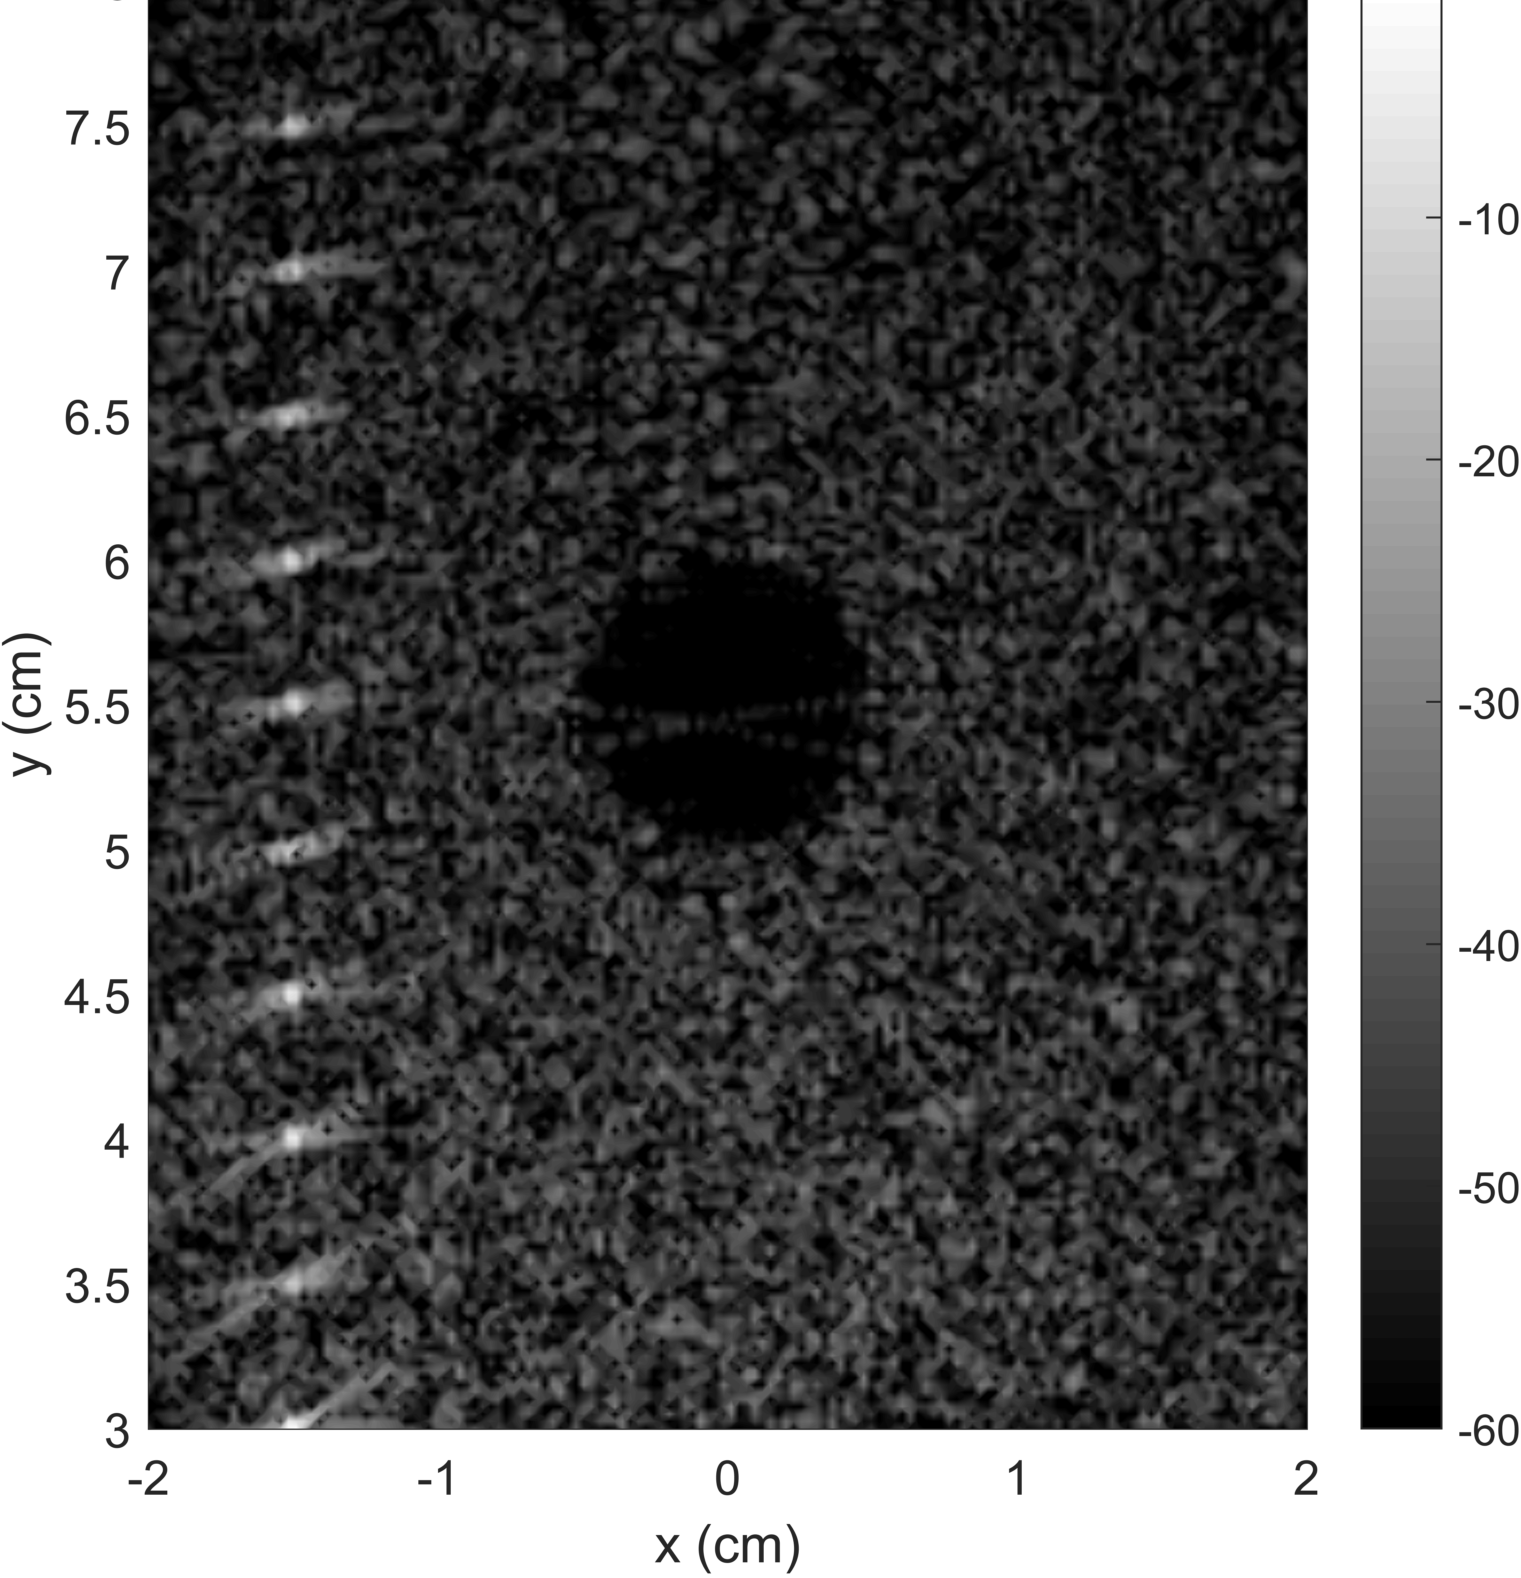
\includegraphics[width=\CIRSFigWidth]{figures/Cyst_pht1.png}}
	\newlength{\pointFigWidth} \setlength{\CIRSFigWidth}{0.4\textwidth}
	\newlength{\pointFigHeight}
	\settoheight{\pointFigHeight}{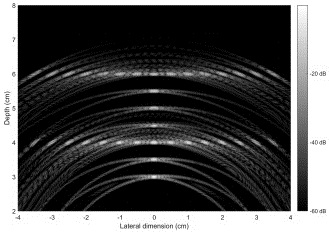
\includegraphics[width=\CIRSFigWidth]{figures/Image_IUS_2017_1.jpg}}
	\begin{figure}
		% Maximum length
%		\subcaptionbox{Reference }{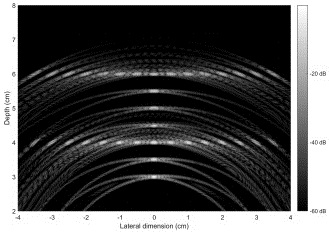
\includegraphics[height=\pointFigHeight]{figures/Image_IUS_2017_1.jpg}}
%		\hfill%
%		\subcaptionbox{CS reconstruction }{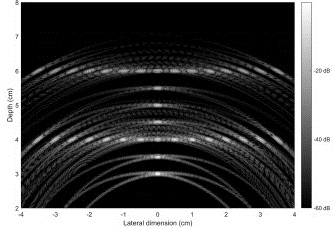
\includegraphics[height=\pointFigHeight]{figures/Image_IUS_2017_2.jpg}}
		\subcaptionbox{Field II simulation }{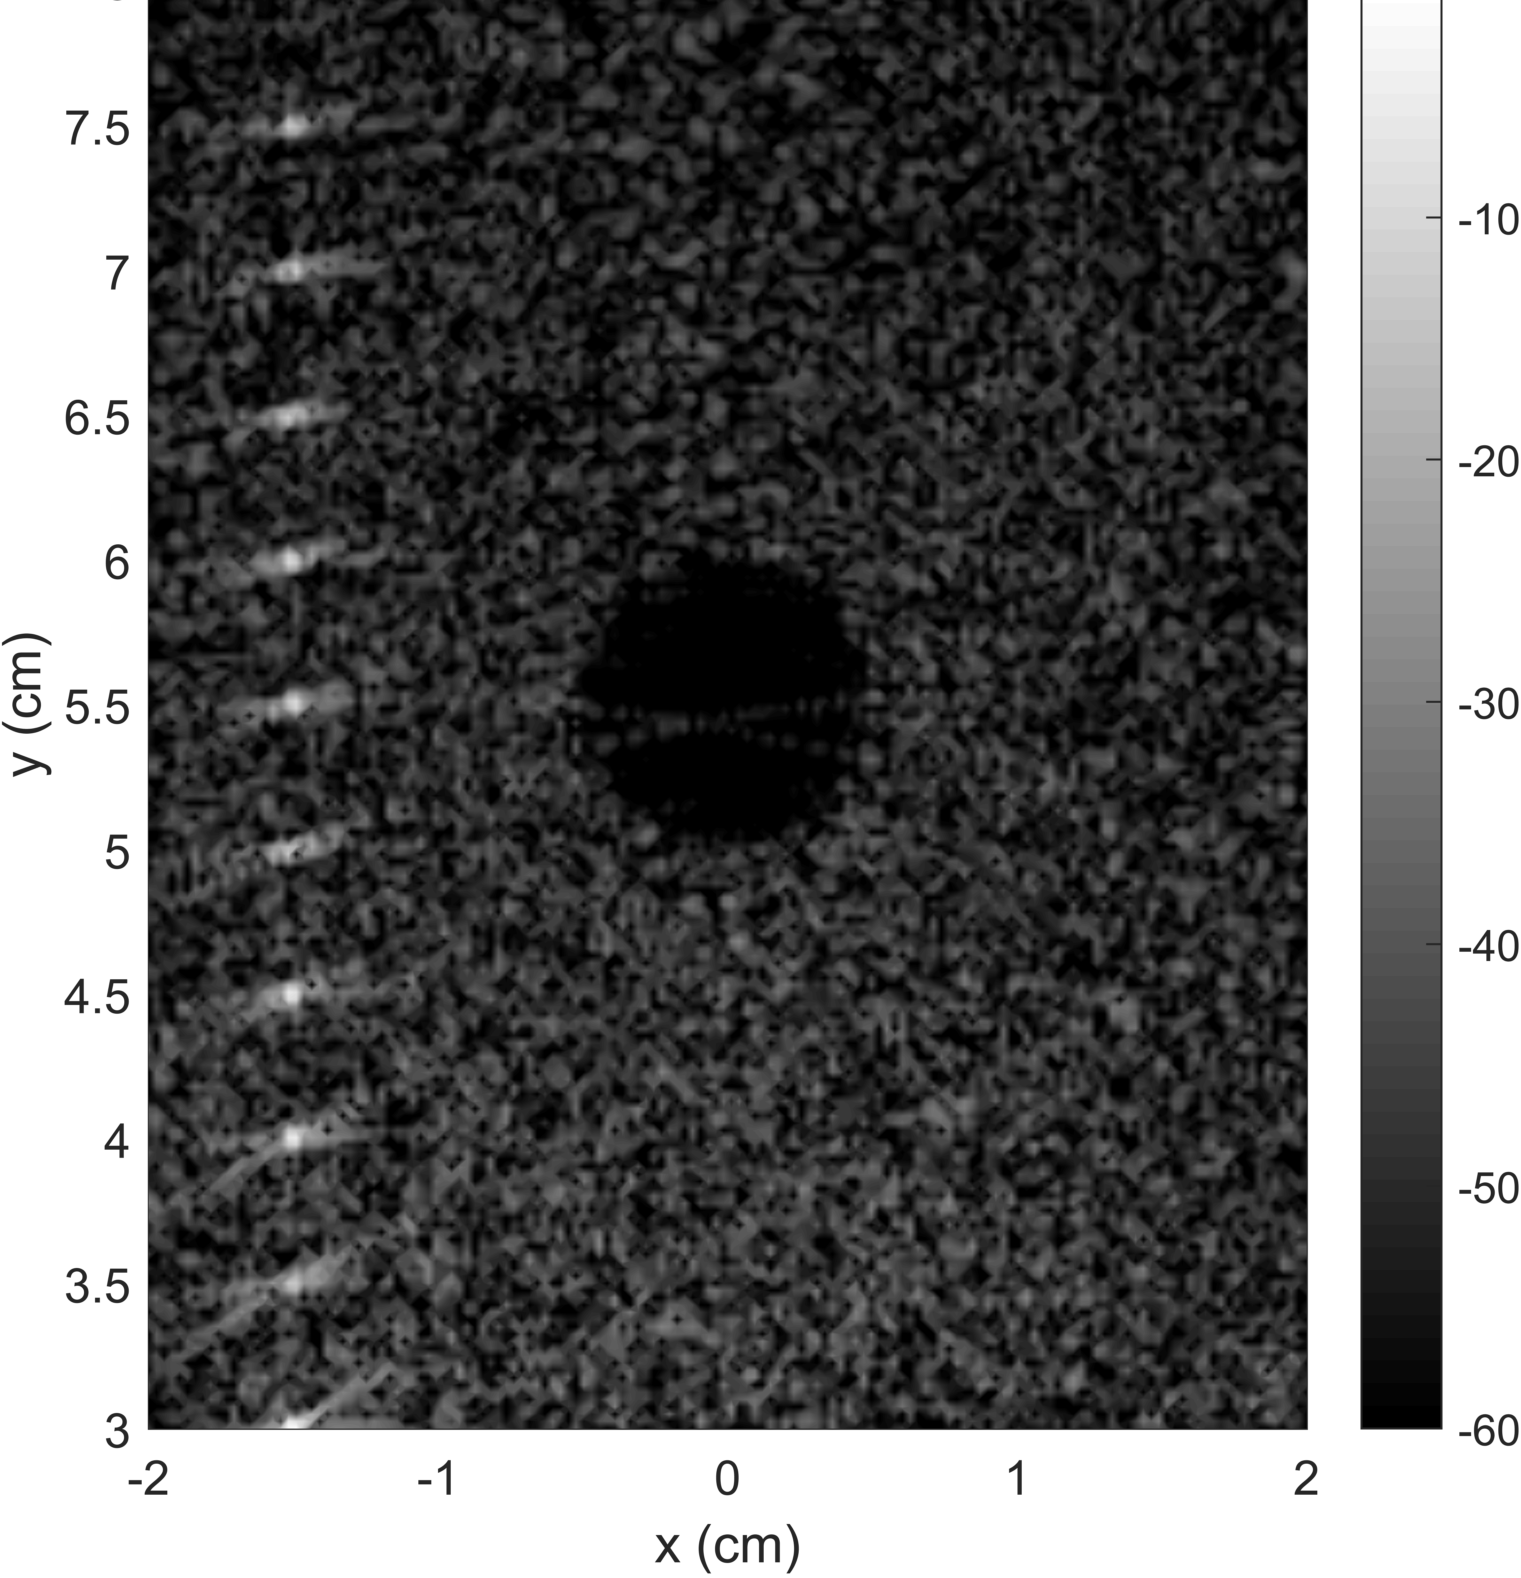
\includegraphics[height=\CIRSFigHeight]{figures/Cyst_pht1.png}}
		\hfill%
		\subcaptionbox{PSF model }{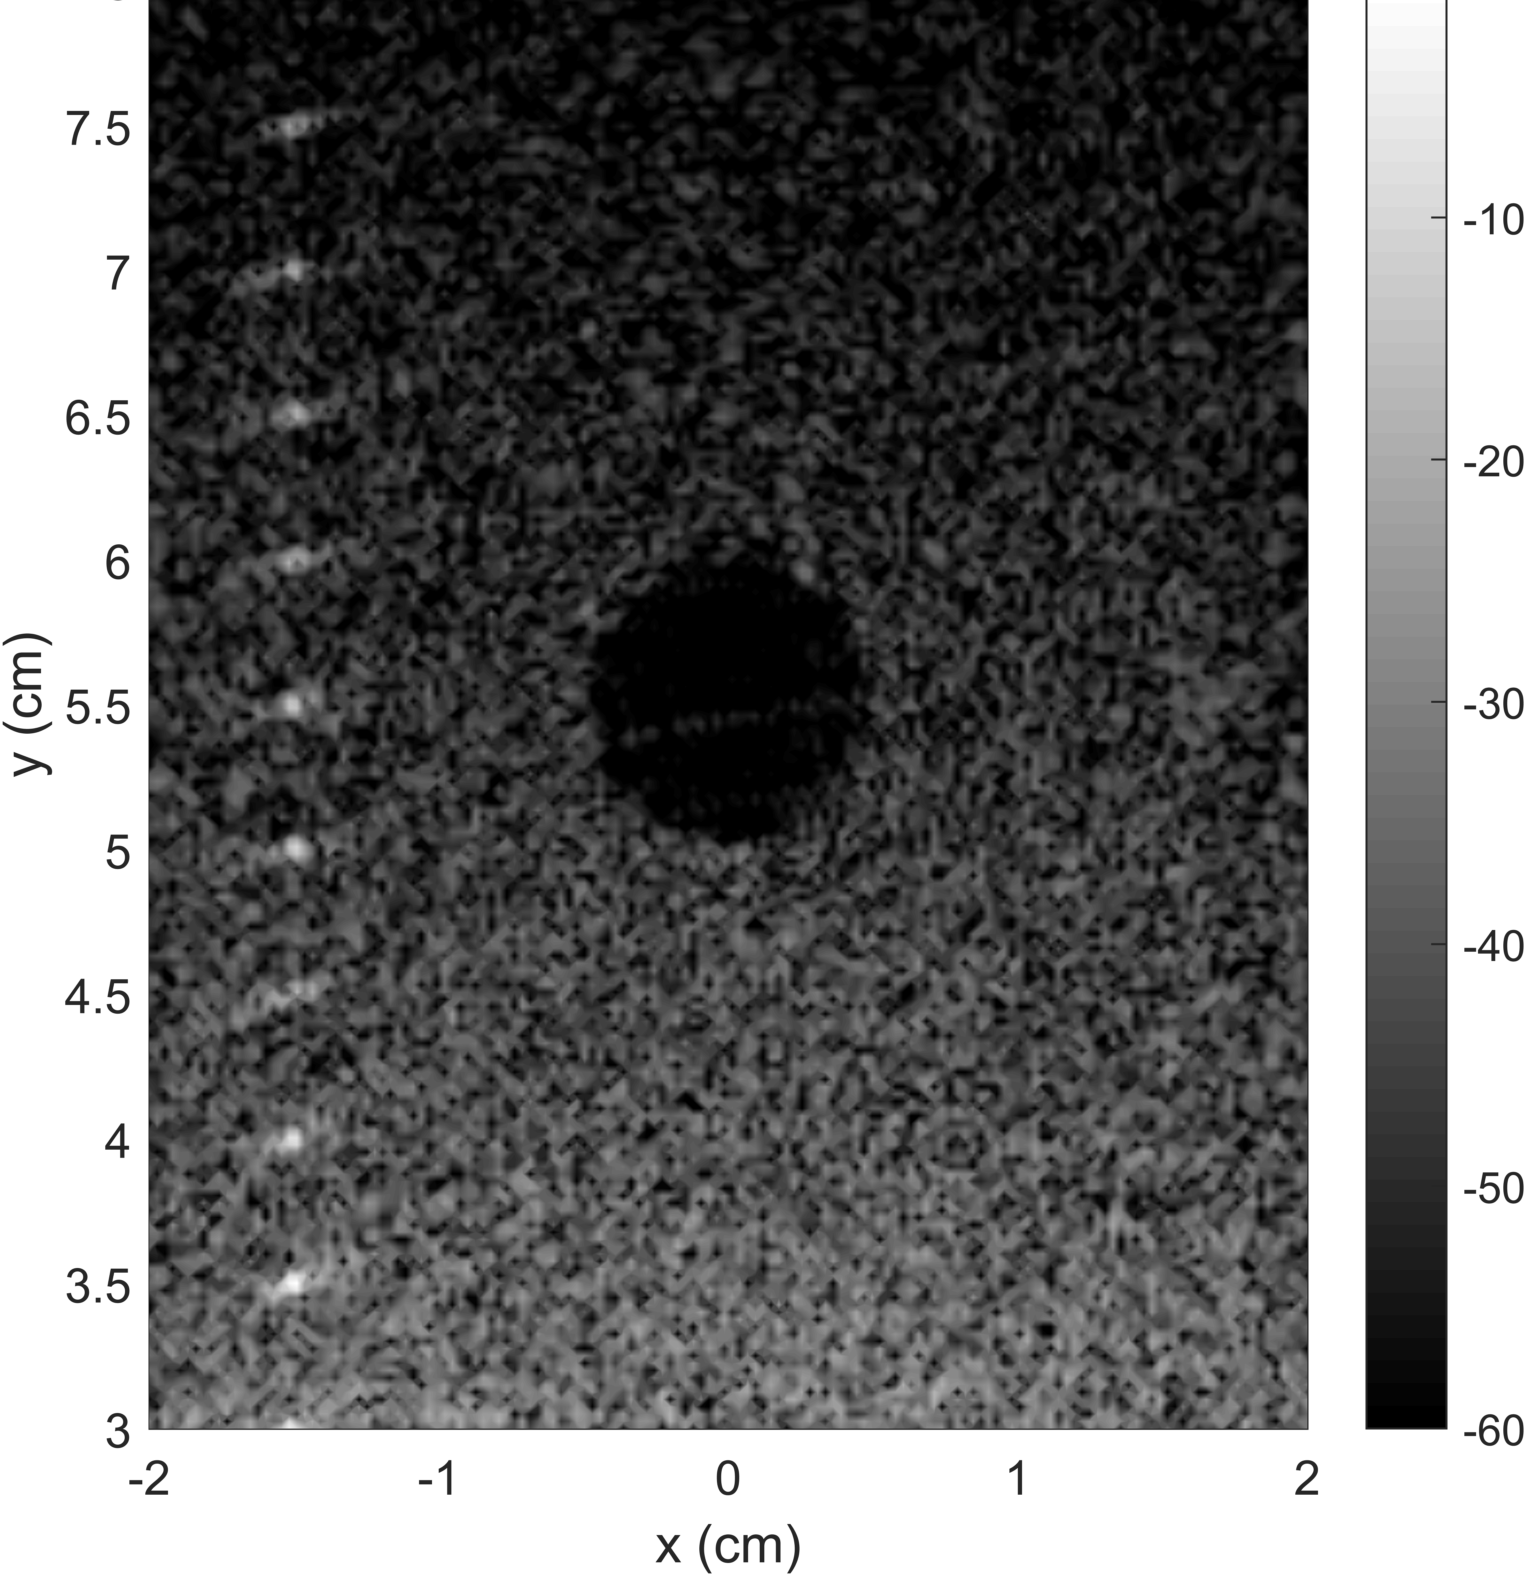
\includegraphics[height=\CIRSFigHeight]{figures/Cyst_pht2.png}}
		\hfill%
		\caption{B-mode image reconstructed from (a) Field II simulation and (b) the proposed PSF model}
	\end{figure}
\end{block}
}%
		\end{column} % End of the first column

		\AddBlankColumn{\BlankColumnWidthCenter} % Empty spacer column

		\begin{column}{\RightColumnWidth} % The second column
			\vbox to \myposterheight{%

%----------------------------------------------------------------------------------------
%	DECONVOLUTION
%----------------------------------------------------------------------------------------
\begin{block}{Deconvolution of ultrasound images}
	\begin{itemize}
		\item The proposed model relates the low-resolution RF image with the high-resolution TRF 
		\item It can be used for \textbf{deconvolution} \textit{i.e.} to retrieve the TRF from the DAS image 
		\item Let us define the RF image $\vect{s} \in \mathbb{R}^{N_{\Omega}}$ and the unknown TRF $\vect{\gamma} \in \mathbb{R}^{N_{\Omega}}$ over the spatial grid $\Omega = \left\lbrace \ser{\vect{r}}{j}, j = 1, \dots, N_{\Omega}\right\rbrace$
		\item The estimate of the TRF can be expressed from the RF image as:
		\begin{equation}
			\label{eq_deconv_pb}
			\vect{\gamma} \in \arg \min \limits_{\hat{\vect{\gamma}} \in \mathbb{R}^{N_{\Omega}}} \| \hat{\vect{\gamma}} \|_p \textnormal{ subject to } \| \mat{H} \hat{\vect{\gamma}} - \vect{s} \| \leq \epsilon
		\end{equation}
		where $p \in \left]0, 2\right]$ and $\mat{H} \in \mathbb{R}^{N_{\Omega} \times N_{\Omega}}$ is defined by:
		\begin{equation*}
			H_{jk} = PSF \left(\ser{\vect{r}}{j}, \ser{\vect{r}}{k}\right), \; \forall \left(\ser{\vect{r}}{j}, \ser{\vect{r}}{k}\right) \in \Omega^2 
		\end{equation*}
	\end{itemize}
\end{block}
\vfill

%----------------------------------------------------------------------------------------
%	EXPERIMENTAL SETTINGS
%----------------------------------------------------------------------------------------
\begin{block}{Experimental settings}
	\begin{itemize}
		\item Comparison with state-of-the-art deconvolution approaches which use spatially-invariant PSF~\cite{Chen2015}
		\item Raw-data simulated on Field II:
		\begin{itemize}
			\item 64-elements phased-array
			\item Central frequency $f_c$ = \SI{2.5}{\mega\hertz}, bandwidth of \SI{80}{\percent} 
			\item Sampling frequency $f_s$ = 
		\end{itemize}
		\item Standard DAS algorithm used to obtain the RF image
		\item Problem~\eqref{eq_deconv_pb} solved with Alternating direction method of multipliers~(ADMM)~\cite{Boyd2010} with $p=1$
	\end{itemize}
\end{block}
\vfill

%----------------------------------------------------------------------------------------
%	RESULTS
%----------------------------------------------------------------------------------------
\begin{block}{Results: Point-scatterers and foetus phantoms}
	\newlength{\PointFigWidth} \setlength{\PointFigWidth}{0.32\textwidth}
	\newlength{\PointFigHeight}
	\settoheight{\PointFigHeight}{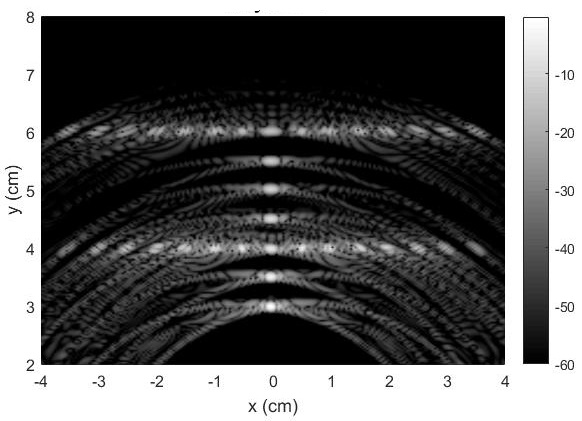
\includegraphics[width=\PointFigWidth]{figures/RF_image.jpg}}
	\newlength{\FoetusFigHeight}
	\settoheight{\FoetusFigHeight}{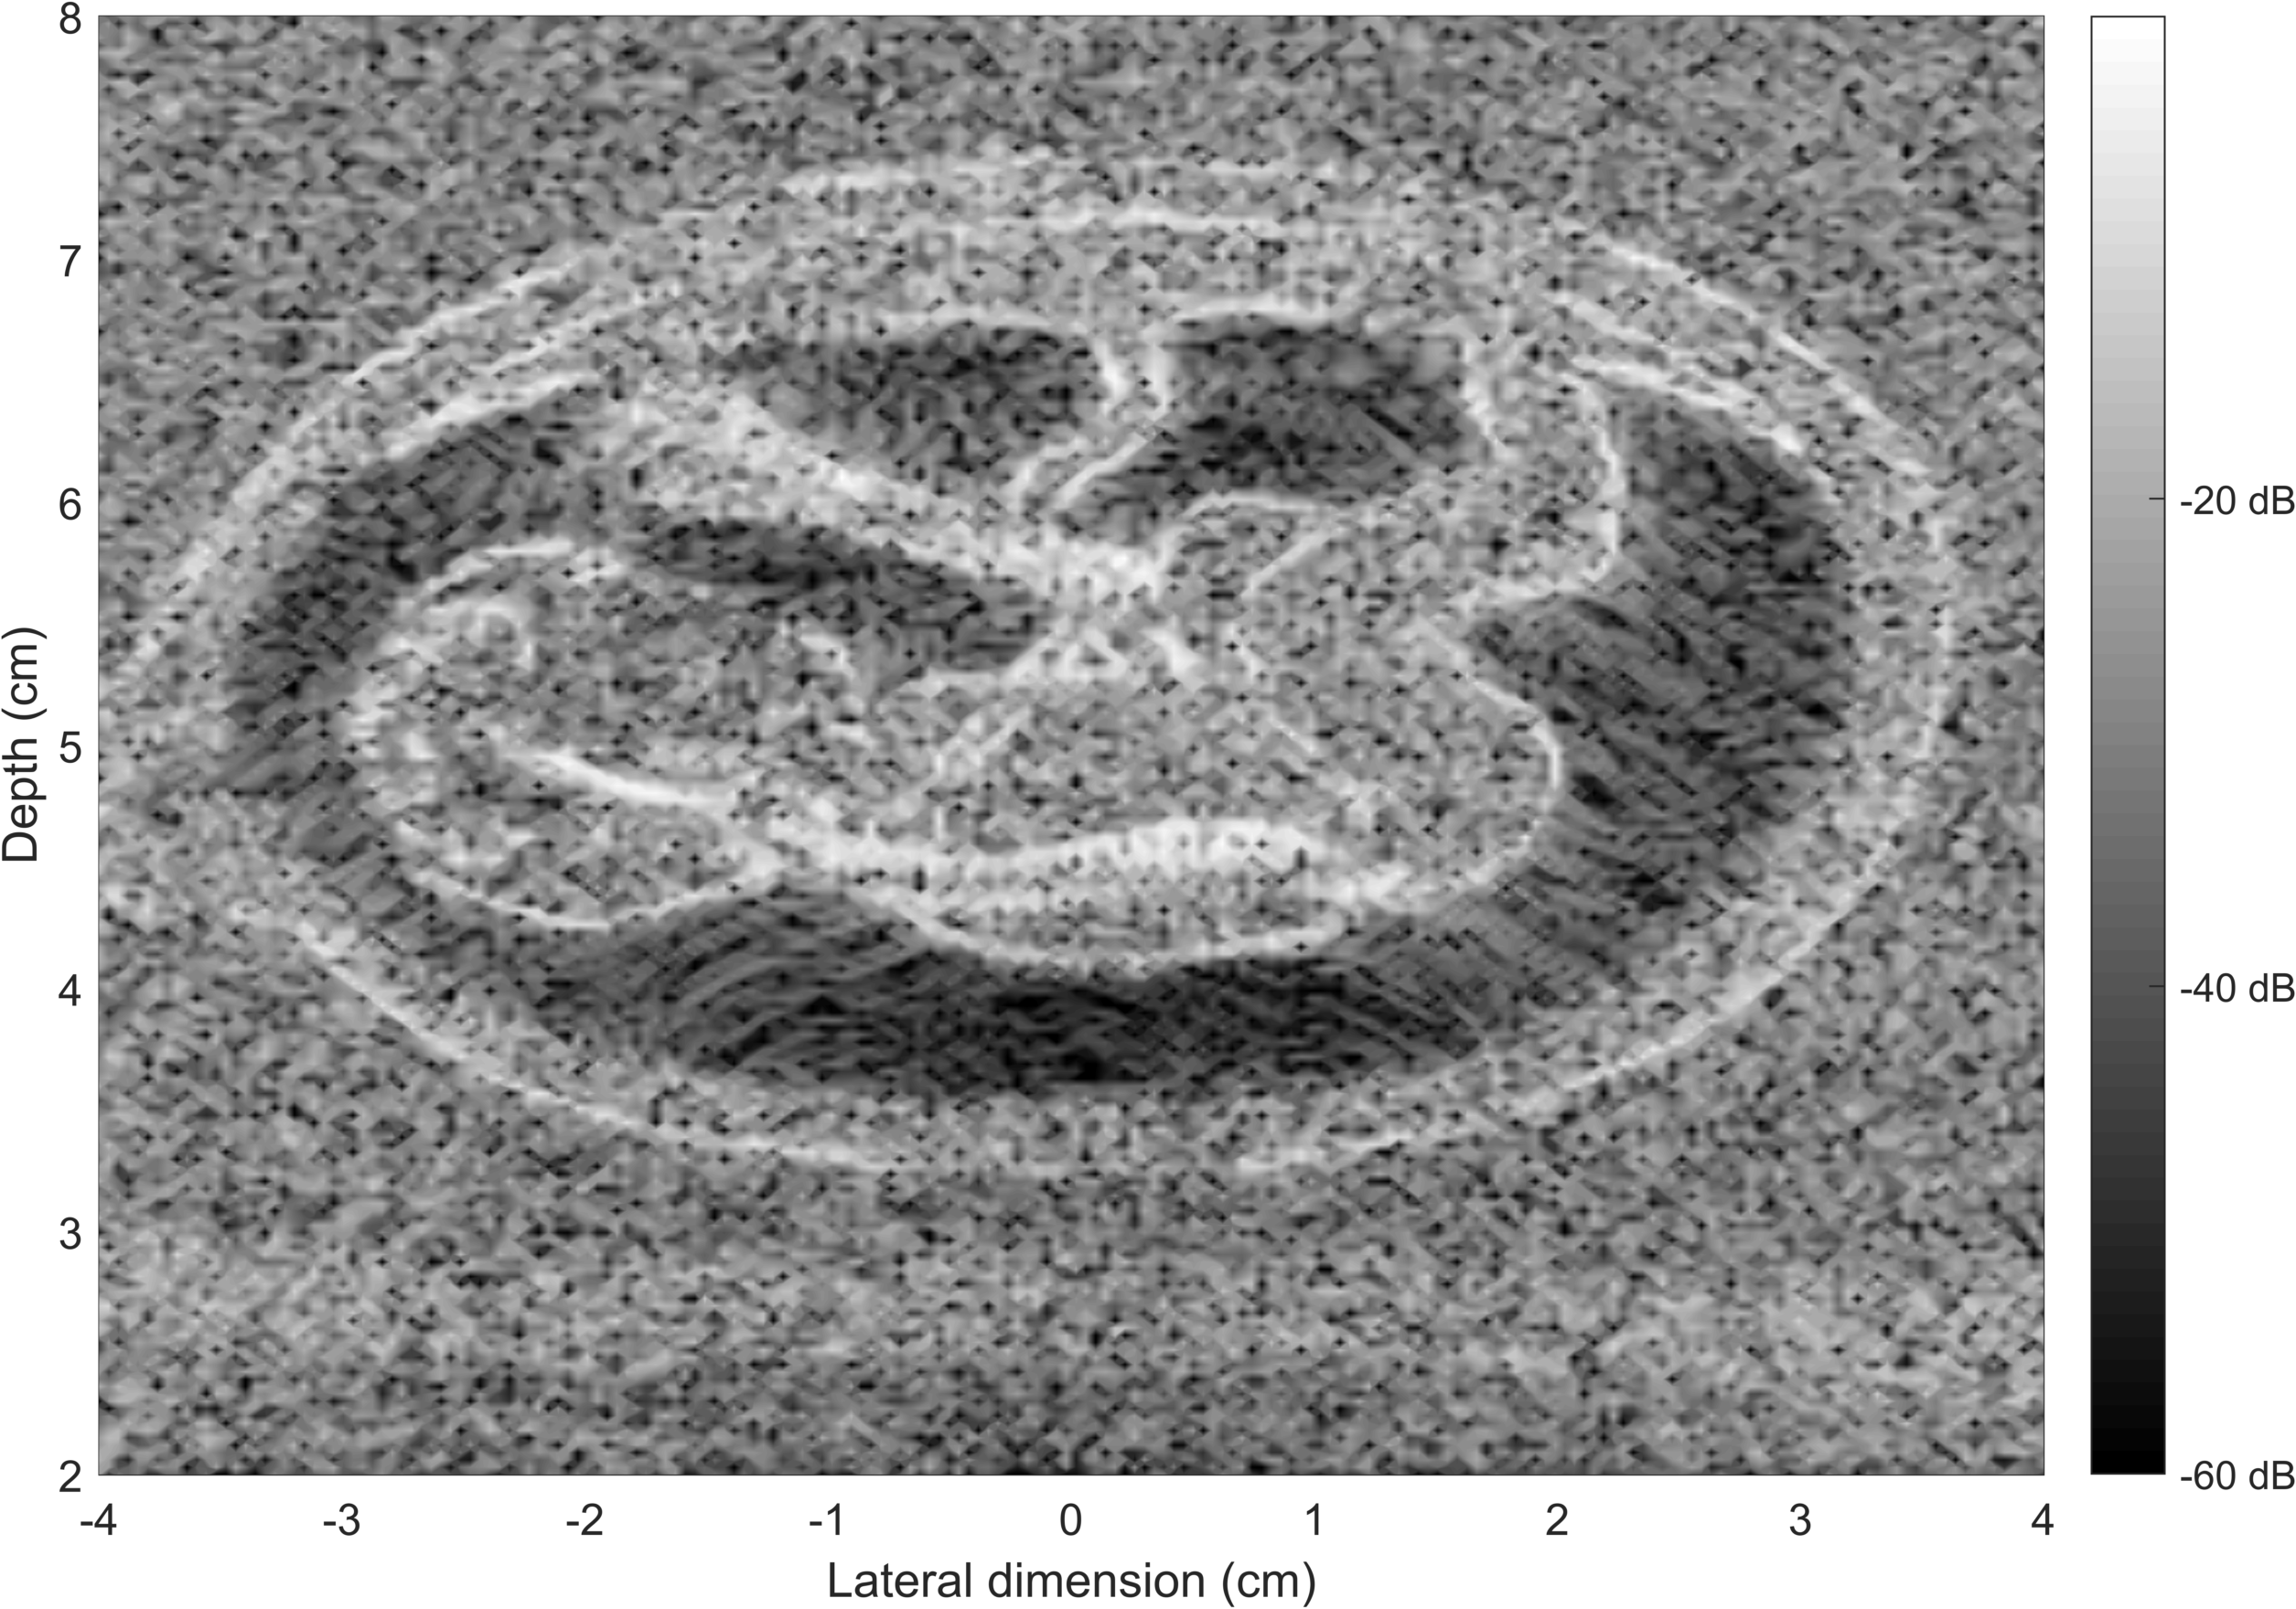
\includegraphics[width=\PointFigWidth]{figures/foetus_example.png}}
	\begin{figure}
		\centering
		% Maximum length
		\subcaptionbox{ }{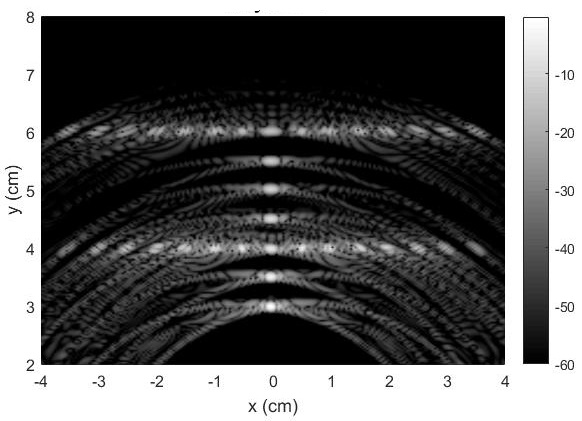
\includegraphics[height=\PointFigHeight]{figures/RF_image.jpg}}
		\subcaptionbox{ }{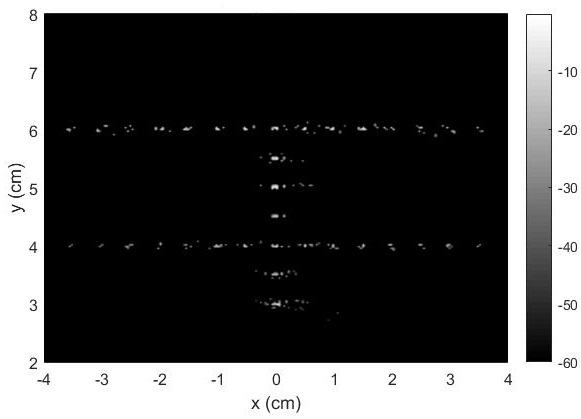
\includegraphics[height=\PointFigHeight]{figures/Deconv_varying_PSF.jpg}}
		\subcaptionbox{ }{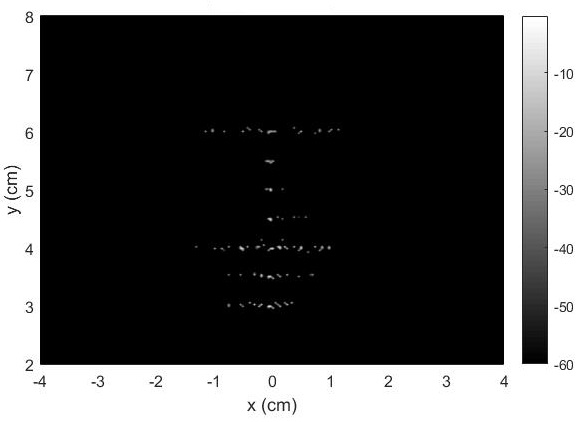
\includegraphics[height=\PointFigHeight]{figures/Deconv_cons_PSF.jpg}}
		~
		\subcaptionbox{ }{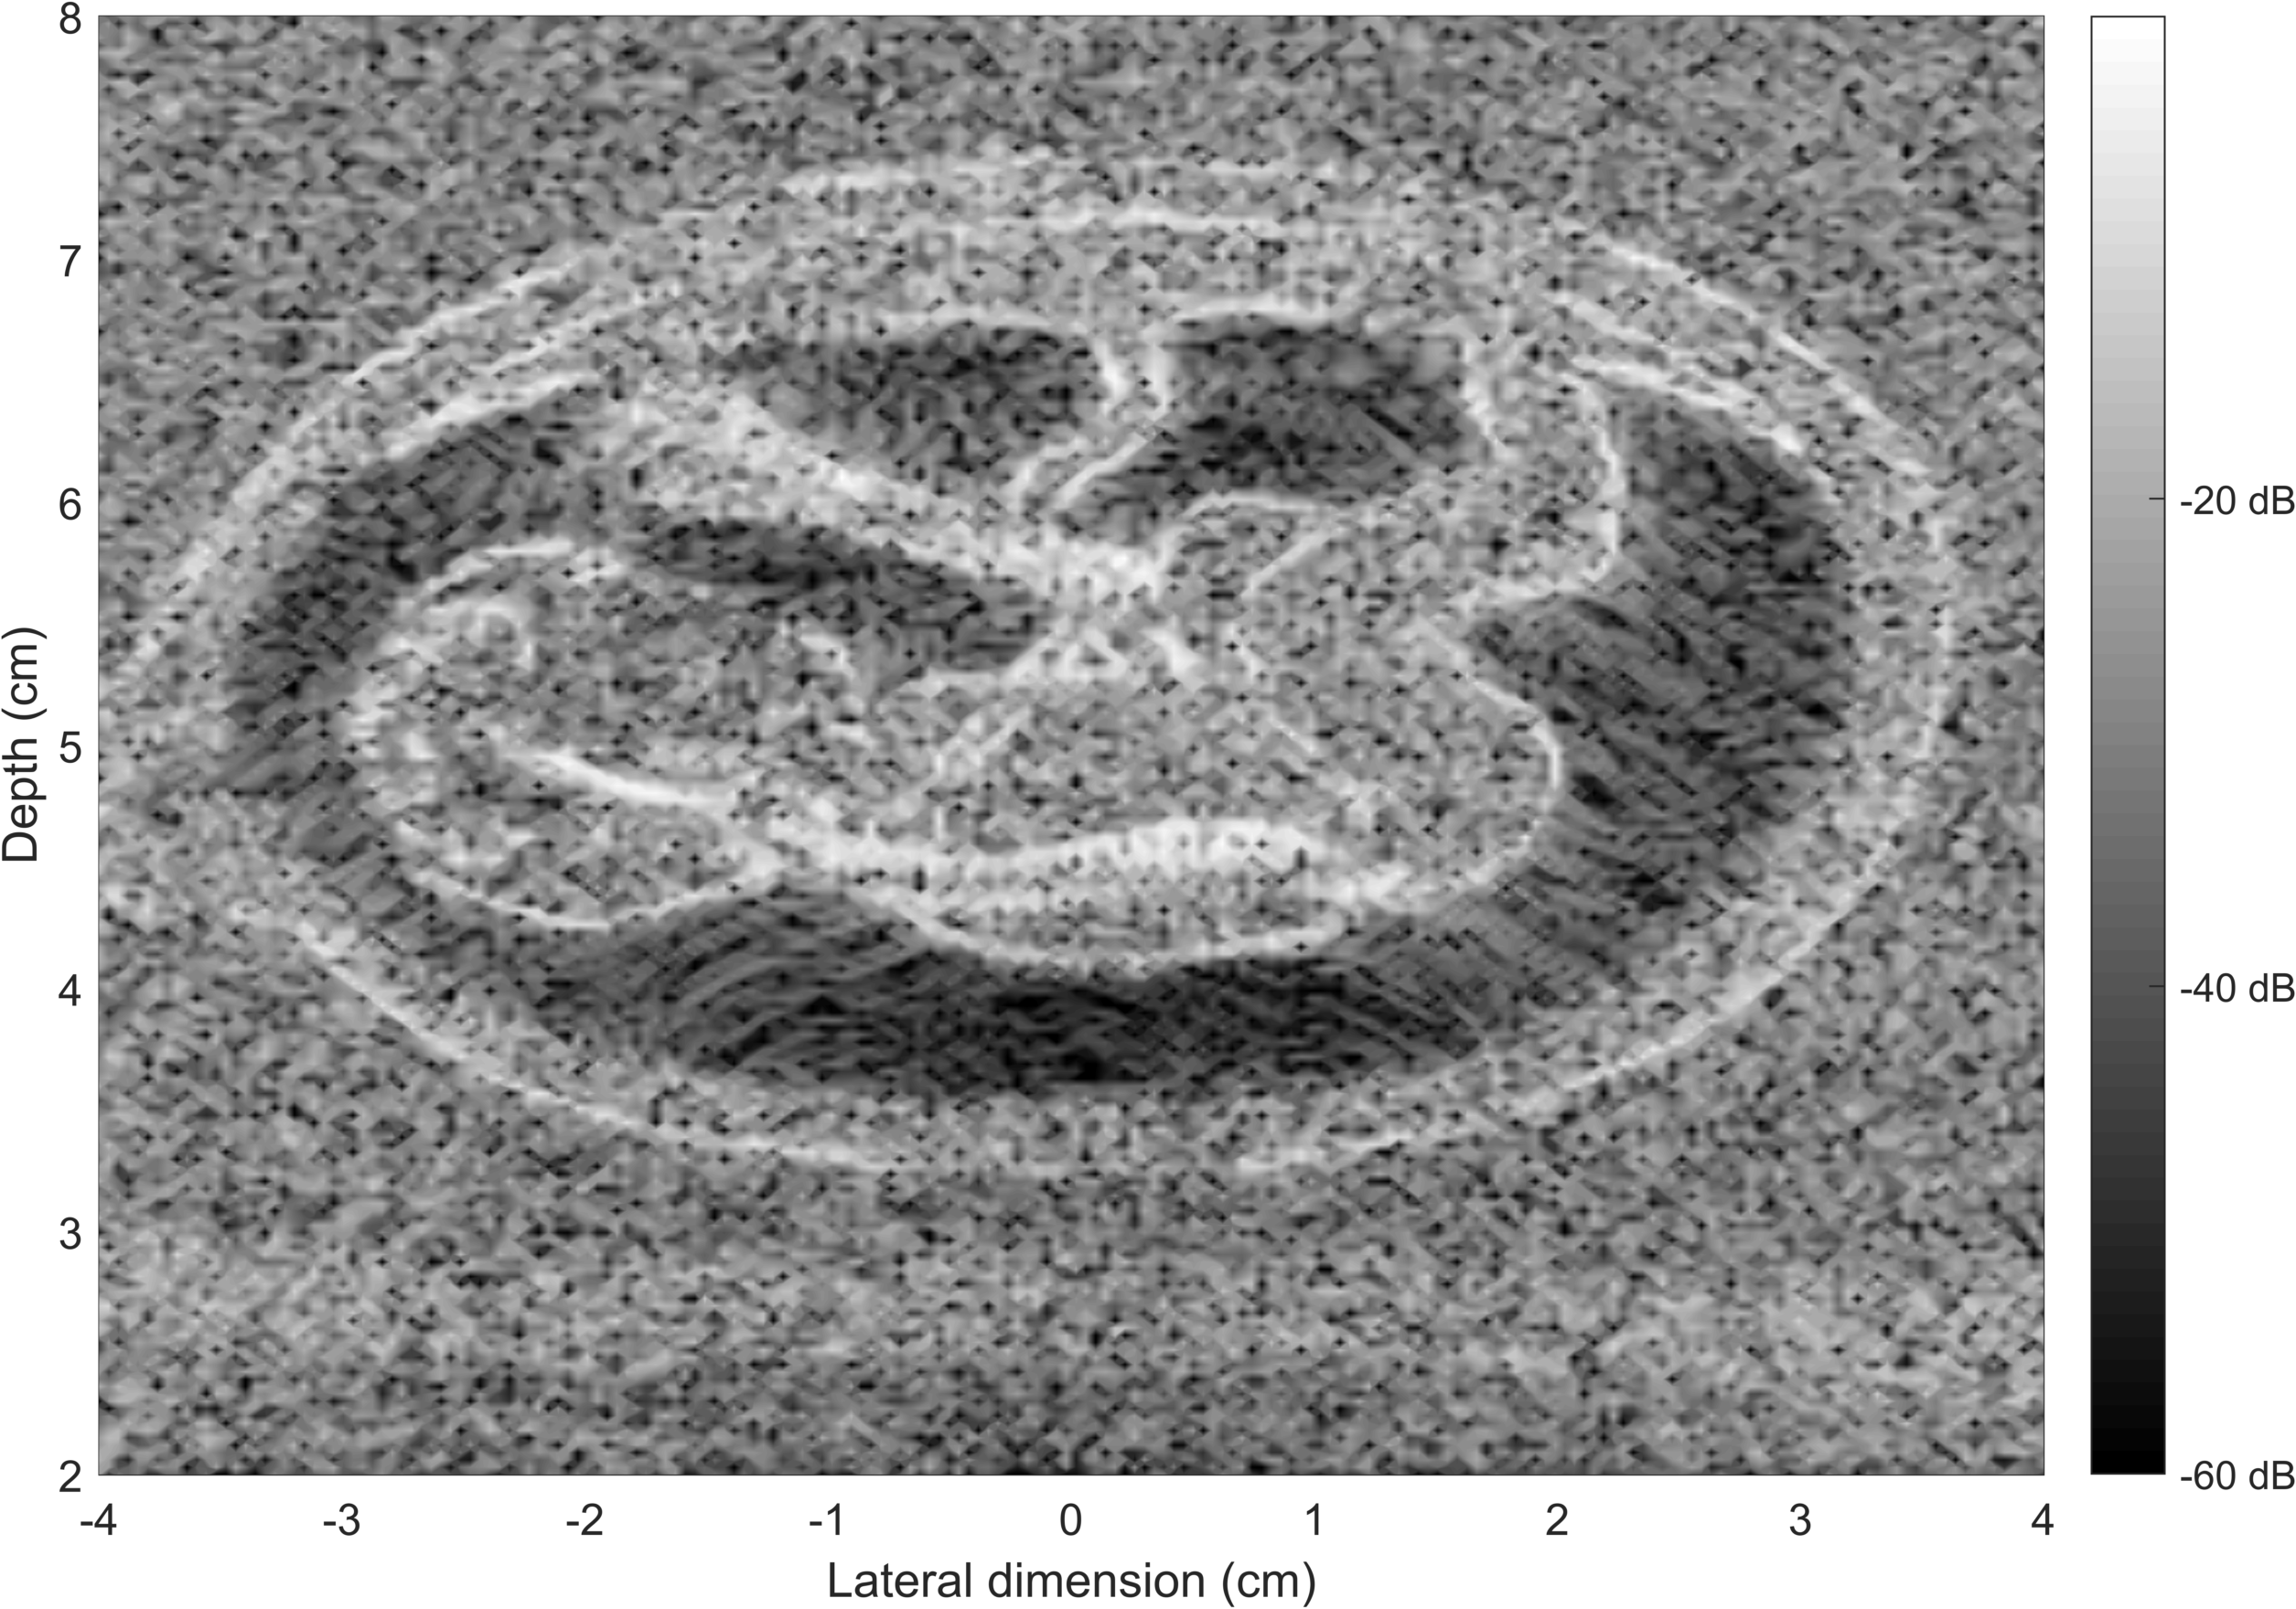
\includegraphics[height=\FoetusFigHeight]{figures/foetus_example.png}}
		\subcaptionbox{ }{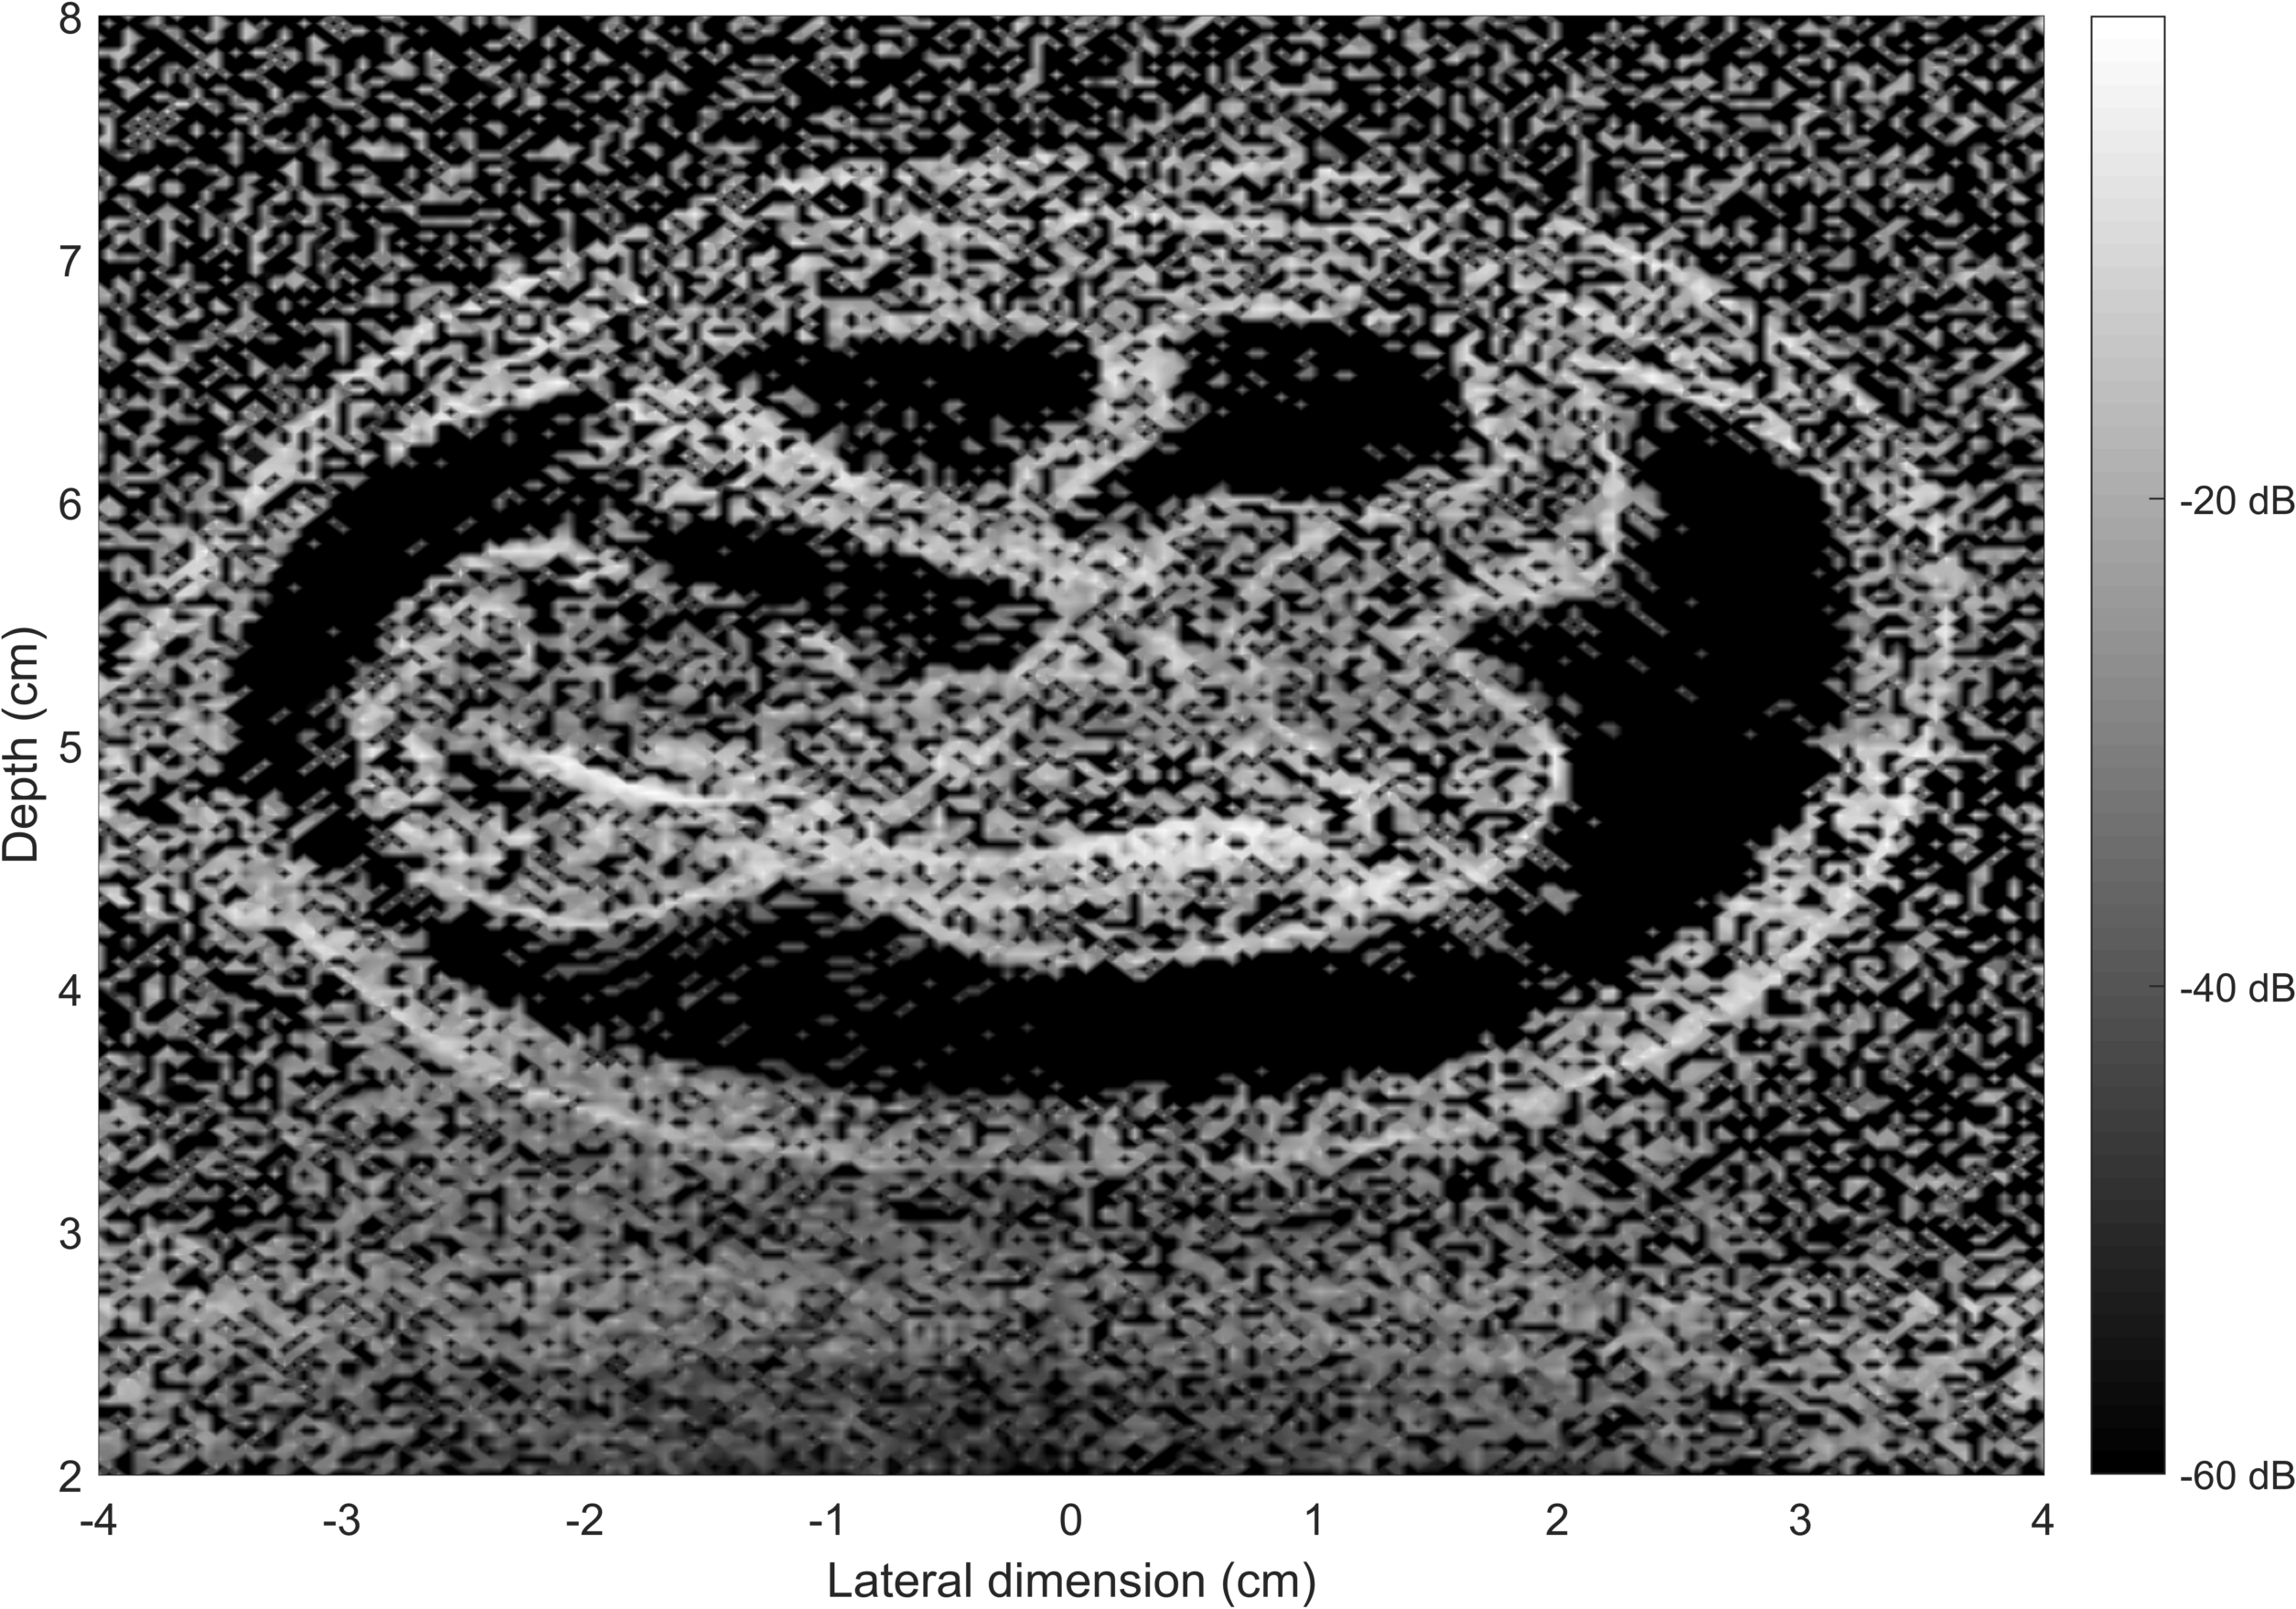
\includegraphics[height=\FoetusFigHeight]{figures/foetus_deconv_var.png}}
		\subcaptionbox{ }{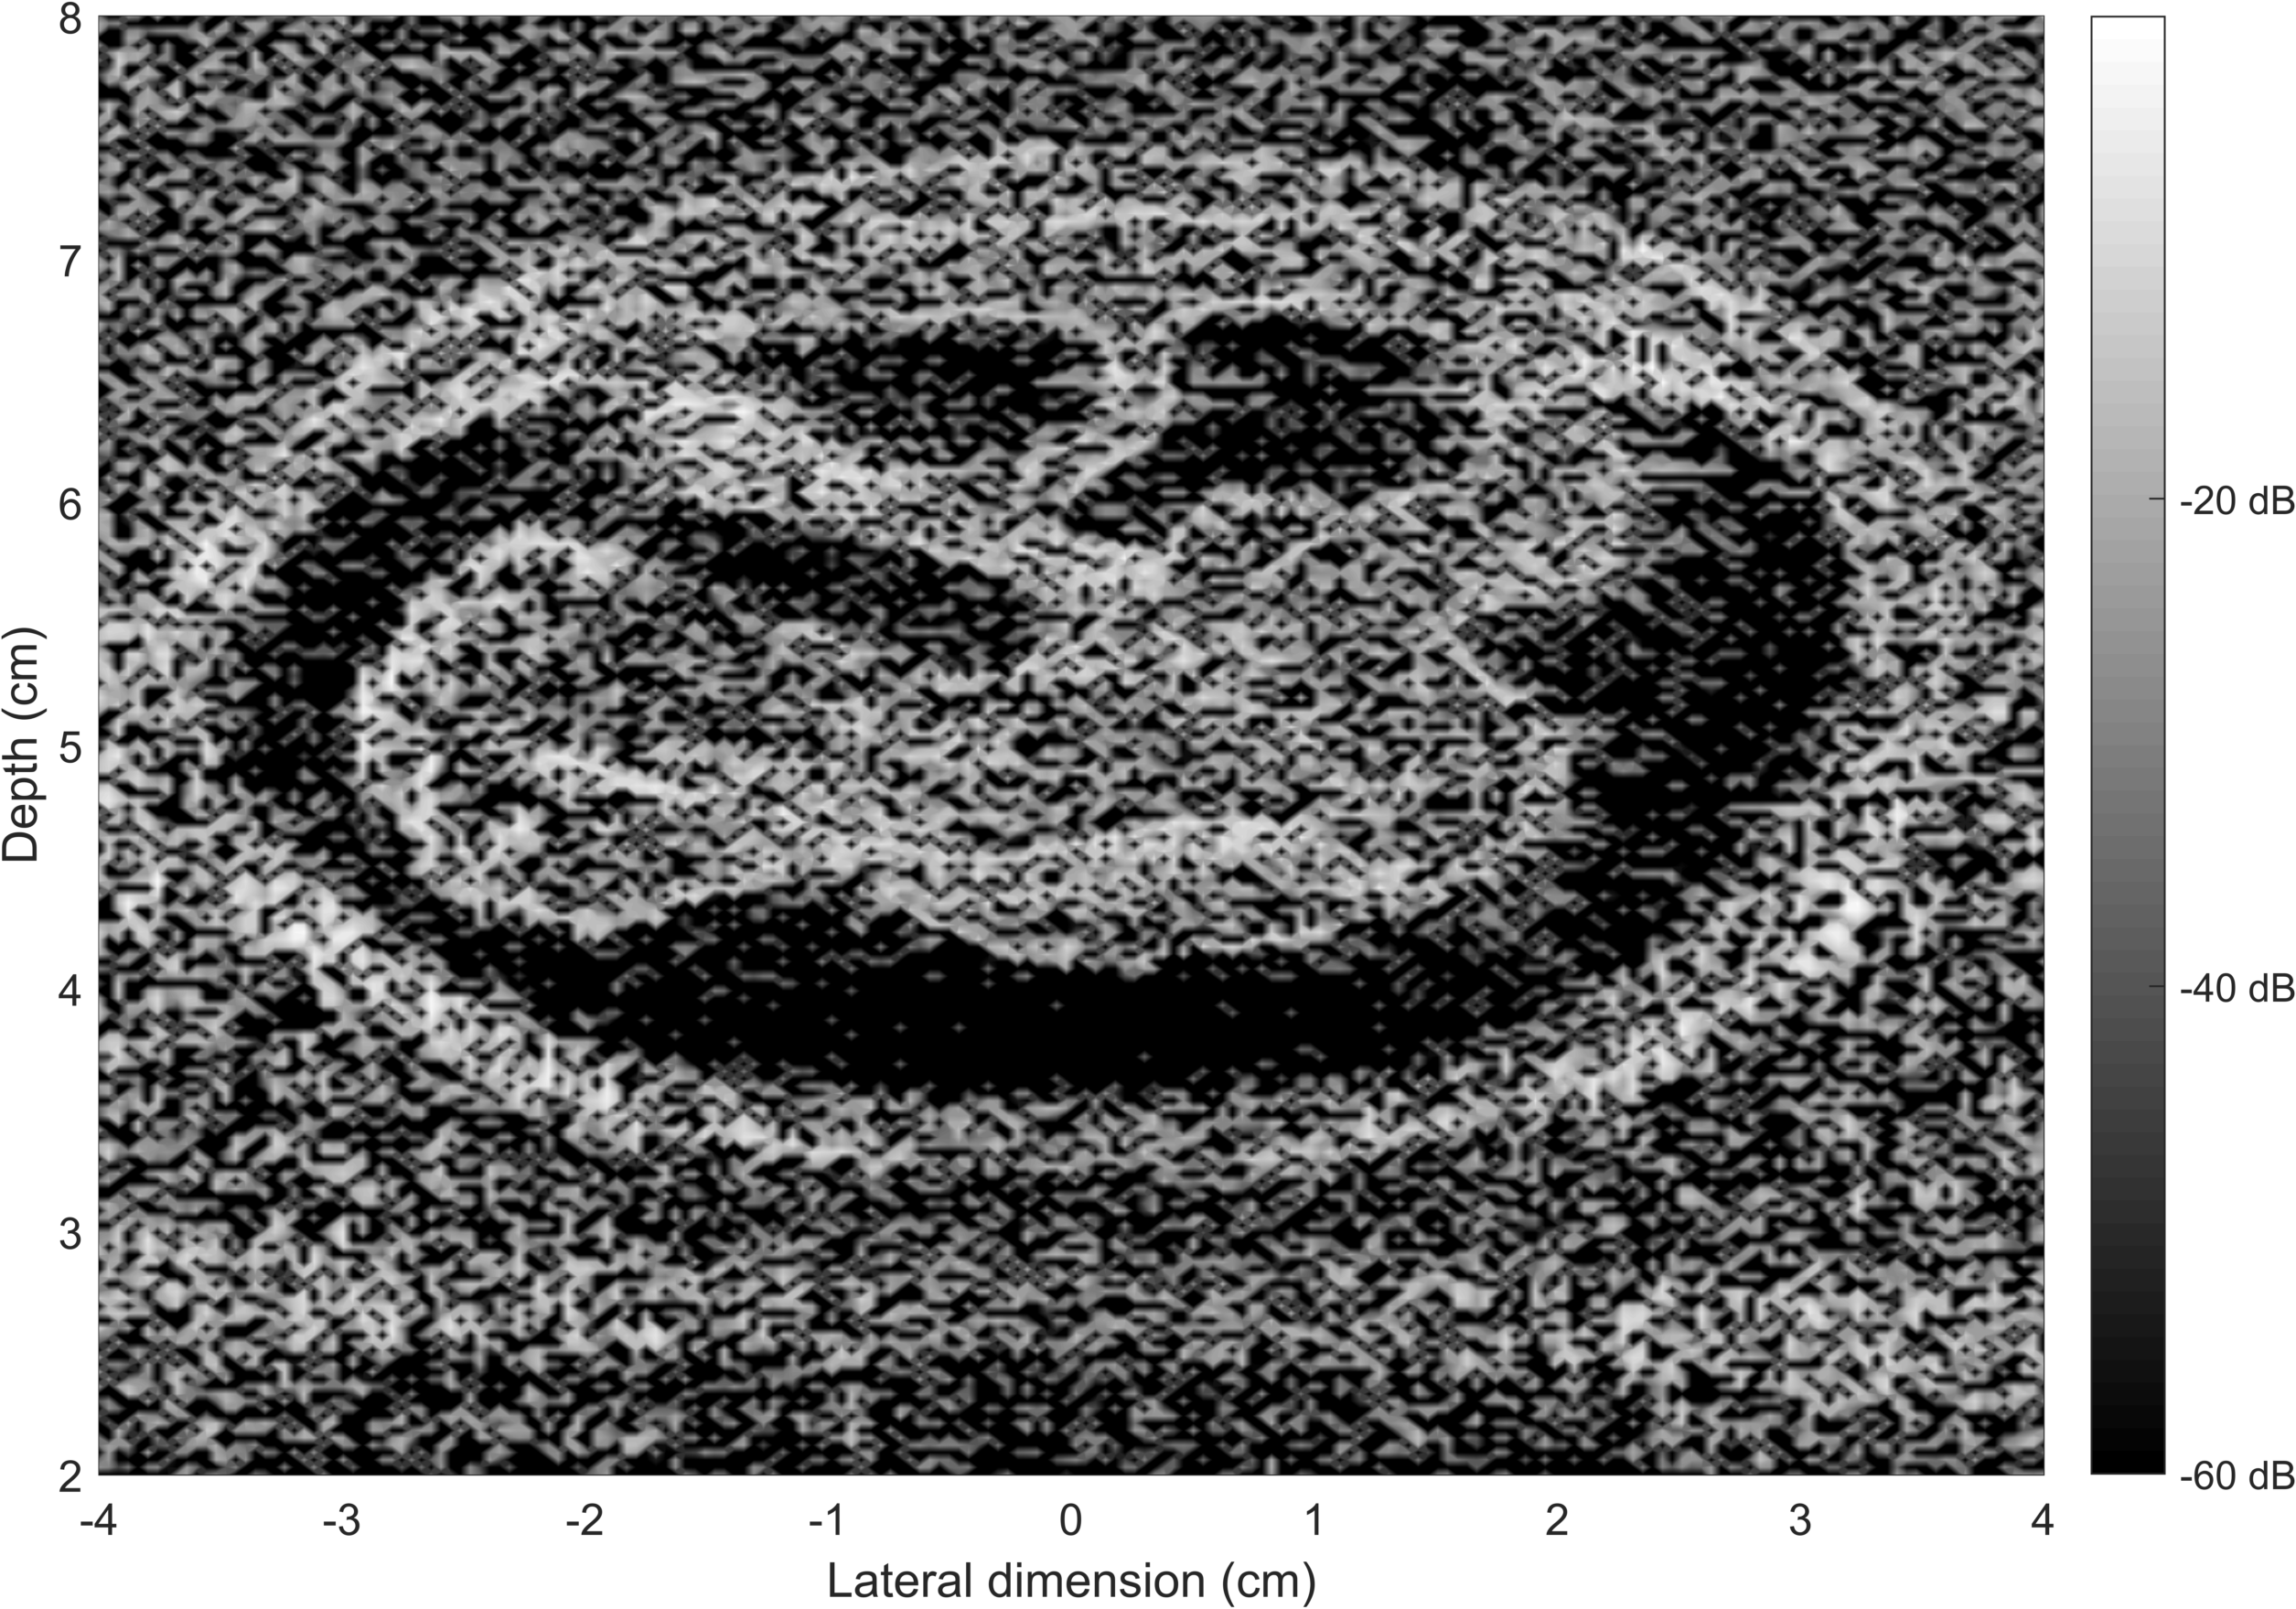
\includegraphics[height=\FoetusFigHeight]{figures/foetus_deconv_cst.png}}
		\caption{(a) RF image of the point-reflectors phantom; (b) Deconvolved image with the proposed operator; (c) Deconvolved image with spatially invariant PSF; (d) RF image of the foetus phantom; (e) Deconvolved image with the proposed operator; (f) Deconvolved image with spatially invariant PSF.}
	\end{figure}

\end{block}
\vfill

%----------------------------------------------------------------------------------------
%	CONCLUSION
%----------------------------------------------------------------------------------------

\begin{block}{Conclusion}
	
\end{block}
\vfill

%----------------------------------------------------------------------------------------
%	BIBLIOGRAPHY
%----------------------------------------------------------------------------------------

\begin{block}{References}
	\printbibliography
\end{block}
}
		\end{column} % End of the second column

		\AddBlankColumn{\BlankColumnWidthRight} % Empty spacer column

	\end{columns} % End of all the columns in the poster

\end{frame} % End of the enclosing frame

\end{document}
